\documentclass[useAMS,usenatbib,fleqn]{mn2e}
\usepackage{amsmath}
\usepackage{amssymb}
\usepackage{graphicx}
\usepackage{caption}
\usepackage{subcaption}
  
\captionsetup{compatibility=false}

\title[Photometric Redshift Estimation]{Photometric Redshift Estimation}
\author[Almosallam et al.]
{\parbox{\textwidth}{Author1,$^1$\thanks{E-mail: ibrahim.almosallam@some.ox.ac.uk} 
Author2,$^{2}$ etc.
} 
\vspace{0.4cm}\\ 
\parbox{\textwidth}{
$^1$Oxford Astrophysics, Department of Physics, Keble Road, Oxford, OX1 3RH, UK\\
$^2$Other institution \\
}}

\begin{document}

\date{\today}

\pagerange{\pageref{firstpage}--\pageref{lastpage}} \pubyear{2015}

\maketitle

\label{first page}

\begin{abstract}
In this study, a novel sparse regression model for photometric redshift estimation is presented which directly target the requirements for the Euclid Space Mission. Data from a synthesised survey was used to train and test the proposed models. We show that approaches which include careful data preparation and model design, a significant improvement can be achieved when compared with several off the shelf machine learning algorithms. Standard implementation of most regression algorithms has as objective the minimisation of the sum of squared errors. This induces a bias in the posterior mean of the output distribution which can be problematic. In this paper we directly optimise the Euclid mission requirement and compare this with other objective functions, such as minimising the maximum error and maximising the number of data points with a predictive error less than a threshold. The results are compared with other popular machine learning algorithms in the field such as ANNz, stableGP and SPGP. The proposed reached a $\Delta z = 0.0085(1+z)$ for a redshift range of $0.2 < z < 2$, exceeding the requirement for the Euclid mission of $\Delta z = 0.05(1+z)$ for the same redshift range.

\end{abstract}

\begin{keywords}
methods: data analysis -- galaxies: distances and redshifts
\end{keywords}

\section{Introduction}
We introduce a novel sparse kernel regression model that greatly reduces the number of basis functions required to model the data. This is achieved by allowing each kernel to have its own hyper-parameters, governing its shape. This is in contrast to the standard kernel-based model in which a set of global hyper-parameters are optimised. The complexity cost of such a kernel-based regression model is $O(n^{3})$, where $n$ is the number of basis functions. This cubic time complexity arise from the cost of inverting an $n$ by $n$ covariance matrix. In a basic Gaussian Process model (GP) \cite{rasmussen+williams}, seen as a kernel regression algorithm, we may regard the basis functions, as the $n$ points in the training set. This renders such an approach unusable for many large-data applications where scalability is a major concern. Much of the work done to make GPs more scalable \cite{sparseGPcitations} is either to make the inverse computation faster or use smaller representative sample to compute the covariance. Examples of the former includes methods such as structuring the covariance matrix such that it is much easier to invert \cite{}, using Toeplitz and Kronecker decomposition for example, or inverse approximation as an optimisation problem \cite{}. To reduce the number of representative points, an $m \ll n$ subset of the training set can be selected which maximises the accuracy or the numerical stability of the inversion. Alternatively, one may search for ``pseudo'' points not necessarily present in the training set to use as basis for the covariance matrix such that it maximises the log marginal likelihood \cite{}. The focus in this paper is on sparse GP modelling where we extend the sparse pseudo GP method using less, but more flexible kernels. Moreover, a weighting scheme is modelled as an integral part of the process to remove, or introduce, any systematic bias to the model. The results are demonstrated on photometric redshift estimation for the Euclid Space Mission. In particular, we use the weighting scheme to remove any distribution bias and introduce a linear bias to directly target the mission's requirement. The proposed approach reached a $\Delta z = 0.0085(1+z)$ on a simulated catalogue, far exceeding the mission's requirement of $\Delta z = 0.05(1+z)$ The paper is organised as follows, a brief introduction to Gaussian Processes for regression and sparse GPs are presented in sections \ref{sec-gaussian-process} and \ref{sec-sparse-gaussian-process},  then the proposed approach is laid out in Section \ref{sec-proposed-approach}. The data set description and experiments are provided in Sections \ref{sec-dataset} and \ref{sec-experiments} respectively. We summarise and conclude in Section \ref{sec-conclusion}.

\textit{TO ADD: The contributions of this paper are as follows....}

\section{Gaussian Processes}
\label{sec-gaussian-process}
In many modelling problems, we have little prior knowledge of the explicit functional form of the function which maps our observable variables into the variable of interest. Imposing, albeit sensible, parametric models, such as polynomials, makes a tacit bias. For this reason, much of modern function modelling is performed using \emph{non-parametric} techniques. For regression, the most widely used approach is that of \emph{Gaussian Processes}.
A Gaussian Process is a supervised non-linear regression algorithm that makes few explicit \emph{parametric} assumptions about the nature of the function fit. For this reason, Gaussian Processes are seen as lying within the class of Bayesian non-parametric models. The main underlying assumption in a GP is that the joint probability of the input variable $x$ and the output variable $y$ is a multivariate Gaussian with mean $\mu=\begin{bmatrix} \mu_{x}\\ \mu_{y}\end{bmatrix}$ and covariance $\Sigma=\begin{bmatrix}\Sigma_{xx} & \Sigma_{xy}\\\Sigma_{yx} & \Sigma_{yy} \end{bmatrix}$, where $\Sigma_{xy}=(x-\mu_{x})(y-\mu_{y})^{T}$. The input variables $x$ is an $n$ by $d$ matrix, where $n$ is the number of data points and $d$ is the dimensionality of the input. Without loss of generality, the output variable $y$ is assumed to be a vector of length $n$ of target outputs but the same concept holds for multiple variable output.

\begin{equation}
p\left ( x,y\right) \sim \mathcal{N} \left ( \begin{bmatrix}\mu_{x}\\\mu_{y} \end{bmatrix}, \begin{bmatrix}\Sigma_{xx} & \Sigma_{xy}\\\Sigma_{yx} & \Sigma_{yy} \end{bmatrix}\right )
\end{equation}

The mean and covariance of the conditional probability $p(y|x)$ therefore is Gaussian distributed as follows:
\begin{equation}
\begin{array}{rcl}
p(y|x)		&\sim&	\mathcal{N} \left ( \mu, \Sigma \right )\\
\mu		&=&		\mu_{x}+\Sigma_{yx}\Sigma_{xx}^{-1}\left ( y-\mu_{y}\right )\\
\Sigma		&=&		\Sigma_{yy}-\Sigma_{yx}\Sigma_{xx}^{-1}\Sigma_{xy}
\end{array}
\end{equation}

The calculation can be simplified by subtracting the mean of the input and the output variables and assuming a prior mean $\mu_{x}=\mu_{y}=0$ and $\Sigma_{xy}$ redefined as $xy^{T}$. The mean and covariance of the conditional probability $p(y|x)$ can then be rewritten as:

\begin{equation}
\label{eq-conditional-zero-mean}
\begin{array}{rcl}
\mu &=& \Sigma_{yx}\Sigma_{xx}^{-1}y\\
\Sigma &=& \Sigma_{yy}-\Sigma_{yx}\Sigma_{xx}^{-1}\Sigma_{xy}
\end{array}
\end{equation}

For the rest of this paper, the prior mean is assumed to be zero unless otherwise stated. So far, it is assumed that no noise exists in our $y$ observations. It can be shown that assuming some noise $\epsilon \sim \mathcal{N}\left(0,\sigma_{n}^{2}\right)$ on the output variable $y$, yields a the following mean and covariance:

\begin{equation}
\label{eq-mean-variance-noise}
\begin{array}{rcl}
\mu &=& \Sigma_{yx}\left(\Sigma_{xx}+I\sigma_{n}^{2}\right)^{-1}y\\
\Sigma &=& \Sigma_{yy}-\Sigma_{yx}\left(\Sigma_{xx}+I\sigma_{n}^{2}\right)^{-1}\Sigma_{xy}+\sigma_{n}^{2}
\end{array}
\end{equation}

For our current definition of the covariance matrix $\Sigma$, the predictive mean is equivalent to a linear regression model, in fact, one can reach the same conclusion by finding the linear regression model that minimizes the sum of squared errors. In other words, the model that minimizes the sum of squared errors also maximizes the probability of the data. For in depth discussion on Gaussian processes and its Bayesian interpretation, the reader is referred to \cite{}.

Since the solution is entirely defined in terms of inner products of the input space, one can utilize the so called ``kernel trick'' to learn non-linear models by replacing the covariance matrix $\Sigma$ with a covariance function $K$, where $K_{ij} = k(x_{i},x_{j})$.

The kernel function $k$ is defined such that the matrix $K$ will be a positive definite matrix. The concept behind the kernel trick is to compute the covariance matrix of high dimensional mapping of the input into a higher dimensional space without explicitly mapping them to that space. The choice of kernel is largely a modelling decision based on the definition of similarity for a given application. In this paper, the squared exponential kernel defined in \eqref{eq-squared-exponential} is used but the concepts introduced here applies to any other kernel function.

\textit{COMMENT: in general I think a more full description is needed. Reading the above feels like the choice of kernel is arbitrary}

\textit{TO ADD: explain why the SE is used - what assumptions does it impose and what advantages does it have.}

\begin{equation}
\label{eq-squared-exponential}
k(x_{i},x_{j}) = \sigma^{2} \exp \left ( -\frac{1} {2\lambda^{2}} \left \|x_{i}-x_{j}\right\|^{2}\right )
\end{equation}

The hyper-parameters of the squared exponential kernel $\sigma^{2}$ and $\lambda^{2}$ are called the height variance and characteristic length scale respectively. Together with the noise variance $\sigma_{n}^{2}$ define the set of hyper-parameters for the GP model. The optimal set of hyper-parameters are the set of values that maximizes the probability of the data given the model, which can be achieved by maximizing the log marginal likelihood defined in \eqref{eq-log-marginal-likelihood} 

\begin{align}
\label{eq-log-marginal-likelihood}
\log\text{ }p(y|x) &= -\frac{1}{2}y^{T}\left(K+I\sigma_{n}^{2} \right)^{-1}y \nonumber \\
&\qquad -\frac{1}{2} \log\left | K+I\sigma_{n}^{2}\right|-\frac{n}{2}log(2\pi)
\end{align}

The search for the optimal set of hyper-parameters is done using gradient search optimization by taking the derivatives of the log marginal likelihood with respect to each hyper-parameter and following the direction of the gradient.

\section{Sparse Gaussian Process}
\label{sec-sparse-gaussian-process}
Gaussian processes are often described as non-parametric regression models due to the analytical nature of its solution and its use of very limited number of hyper-parameters that live in the kernel. However, GP regression can also be viewed as feature transformation methods $x\in \mathbb{R}^{d}:\rightarrow K\in \mathbb{R}^{n}$ parameterized by the data and the kernel function followed by linear regression, or optimizing the following objective:

\begin{equation}
\label{eq-linear-regression-objective}
\begin{array}{lcl}
\underset{w}{\text{min}} &\frac{1}{2}\left ( Kw-y \right )^{T}\left( Kw-y \right )+\frac{1}{2}\sigma_{n}^{2}w^{T}w
\end{array}
\end{equation}

The feature transformation $K$ is essentially describing each data point by how ``similar'' it is to every point in the training set where the similarity measure is defined by the kernel function. Obviously, if two training points are very similar, that will result in very correlated features and thus adding extra computational cost for very little or no added information. Selecting a subset of the training set that maximizes the preserved information is a research question addressed in [x], whereas in [x] the basis functions are treated as an optimization problem rather than a selection problem where their locations are treated as hyper-parameters. The new transformation is now $x\in \mathbb{R}^{d}:\rightarrow K\in \mathbb{R}^{m}$ where $m\ll n$ is the number of basis used. The transformation matrix $K$ will therefore be a rectangular $n$ by $m$ matrix and the solution for $w$ in \eqref{eq-linear-regression-objective} is calculated as follows:

\begin{equation}
\label{eq-linear-regression-objective-rectangular}
w = \left(K^{T}K+I\sigma_{n}^{2} \right)^{-1}K^{T}y
\end{equation}

Even though these models improve the computational cost greatly, very little is done to compensate for the reduction in modeling complexity. The selection method is always bounded by the full GP's accuracy. On the other hand, the sparse GP's ability to place the basis freely across the input space does compensate for the basis set size reduction as they can be better positioned to describe the distribution of the data. However, in both cases a global set of hyper-parameters is used for all basis functions therefore limiting the algorithm's capability to model patterns in the data with the number of basis and their locations. Moreover, the objective in \eqref{eq-linear-regression-objective} by definition minimizes the sum of squared errors, therefore for any non-uniformly distributed output, the optimization routine will bias the model towards the mean of the output distribution and will seek to fit the region of space where there is more data.

In the next section, the proposed method is described which addresses the above issues by defining each basis with its own hyper-parameters to account for variable density and/or pattern across the input space and allows the algorithm to learn more complex models with a fewer number of basis functions. In addition, a weighting mechanism to remove any distribution bias from the model is directly incorporated into the objective.

\section{Proposed Approach}
\label{sec-proposed-approach}

In this paper, we extend the sparse GP approach by modelling each basis with its own set of hyper-parameters, namely the kernel function in \eqref{eq-squared-exponential} is redefined as follows:

\begin{equation}
\label{eq-squared-exponential-extension}
k(x_{i},p_{j}) = \exp{\left(-\frac{1}{2\lambda_{j}^{2}}\left\| x_{i}-p_{j}\right\|^{2}\right)}
\end{equation}

Where $P=\{p_{j}\}_{j=1}^{m}$ is the set of basis coordinates in $\mathbb{R}^{d}$ and $\lambda_{j}$ is the corresponding length scale for basis $j$. Note that the hyper-parameter $\sigma$ has been dropped, as it interferes with the regularization objective. This can be seen from the final prediction equation $f(x_{i},w)=\sum_{j=1}^{m}w_{j}\sigma_{j}^{2}\exp{\left(-\left\| x_{i}-p_{j}\right\|^{2}/2\lambda_{j}^{2}\right)}$, the weights are always multiplied by their associated $\sigma$. Therefore, the optimization process will always compensate for decreasing $w_{j}^{2}$ by increasing $\sigma_{j}^{2}$. Dropping the height variance ensures that the kernel functions do not grow beyond control and delegates learning the linear coefficients and regularization to the weights $w_{j}$. A gradient based optimization is used to find the set of hyper-parameters by computing the derivatives with respect to each variable to find the search direction, specifically we apply a Quasi-Newton optimization using the L-BFGS algorithm \cite{}. The derivative with respect to each length scale and position are provided in equations \eqref{eq-dfdl} and \eqref{eq-dfdp} respectively. 

\begin{subequations}
\begin{align} 
\label{eq-dfdl}
\frac{\partial f(x,w)}{\partial \lambda_{j}} &= \sum_{i=1}^{n}\left(f(x_{i},w)-y_{i}\right)w_{j}K_{ij}\frac{\left\| x_{i}-p_{j}\right\|^{2}}{\lambda_{j}^{3}}\\
\label{eq-dfdp}
\frac{\partial f(x,w)}{\partial p_{jk}} &= \sum_{i=1}^{n}\left(f(x_{i},w)-y_{i}\right)w_{j}K_{ij}\frac{(x_{ik}-p_{jk})}{\lambda_{j}^{2}}
\end{align}
\end{subequations}

Finding the set of hyper-parameters that optimizes the solution, is in effect finding the set of radial basis defined by their positions $p$ and radius $\lambda$ that jointly describes the patterns across the input space, and by parameterizing them differently, the model is more capable to accommodate different regions of the space more specifically. The kernel in \eqref{eq-squared-exponential-extension} can be further extended to, not only model each basis with its own radius $\lambda_{j}$, but also model with its own covariance defined by $C_{j}$. This enables the basis to have any arbitrary shaped ellipses given it more flexibility. The kernel in \eqref{eq-squared-exponential-extension} can be extended as follows:

\begin{equation}
\label{eq-squared-exponential-covariance-extension}
k(x_{i},p_{j}) = \exp{\left(-\frac{1}{2}\left(x_{i}-p_{j}\right)C_{j}^{-1}\left(x_{i}-p_{j}\right)^{T}\right)}
\end{equation}

To make the optimization process faster and simpler, we define the following variables:

\begin{subequations}
\begin{align} 
\label{eq-error}
E &= \left(f(x,w)-y)\right)w^{T}\\
\label{eq-Cinv}
C_{j}^{-1} &= \Lambda\Lambda_{j}^{T}\\
\label{eq-Delta_j}
\Delta_{j} &= \left(x-\underset{n}{1}p_{j}\right)\\
\label{eq-V_j}
V_{j} &= \Delta_{j}\Lambda_{j}
\end{align}
\end{subequations}

Where $\underset{n}{1}$ denotes a column vector of length $n$ with all elements set to 1. Optimizing with respect to $\Lambda_{j}$ directly ensures that the covariance matrix is positive semi-definite and makes it faster from a computational perspective, as the kernel functions for all the points with respect to a particular basis can be computed more efficiently as follows:

\begin{equation}
\label{eq-squared-exponential-covariance-extension-simplified}
k(x,p_{j}) = \exp{\left(-\frac{1}{2}\left(V_{j}\circ V_{j}\right)\underset{d}{1}\right)}
\end{equation}

The symbol $\circ$ denotes the Hadamard product or the element-wise matrix multiplication. The exponent in \eqref{eq-squared-exponential-covariance-extension-simplified} basically computes the sum of squares in each row of $V_{j}$. This allows for a more efficient computation of the kernel functions for all points in a single matrix operation. The derivatives with respect to each $\Lambda_{j}$ and $p_{j}$ are shown in \eqref{eq-dfdL} and \eqref{eq-dfdP}.

\begin{subequations}
\begin{align} 
\label{eq-dfdL}
\frac{\partial f(x,w)}{\partial \Lambda_{j}} &= -\left( \Delta_{j}\circ \left(\left(K_{*,j}\circ E_{*,j}\right)\underset{d}{1}\right) \right)^{T}V_{j}\\
\label{eq-dfdP}
\frac{\partial f(x,w)}{\partial p_{j}} &= \left( K_{*,j}\circ E_{*,j} \right)^{T}V_{j}\Lambda_{j}^{T}
\end{align}
\end{subequations}

Where $K_{*,j}$ is the $j$'th column of matrix $K$, similarly for $E_{*,j}$. The differences between the three approaches using a different number of basis functions are demonstrated on a toy classification example shown in Figure \ref{fig-toy-example} and the results are shown in Figure \ref{fig-toy-comparison}. The class probability distribution clearly show the advantage of having basis functions with more flexibility. 

\begin{figure}
       \centering
       \includegraphics[trim = 25px 12px 10px 10px, clip=true,width=0.75\columnwidth]{clouds.jpg}
        \caption{A toy classification dataset. }       
       \label{fig-toy-example}
\end{figure}
  
\begin{figure}
        \centering
        \begin{subfigure}[b]{70 px}
                \includegraphics[trim = 150px 100px 150px 70px, clip=true,width=\textwidth]{global1.jpg}
        \end{subfigure}
        ~
         \begin{subfigure}[b]{70 px}
                \includegraphics[trim = 150px 100px 150px 70px, clip=true,width=\textwidth]{VL1.jpg}
        \end{subfigure}
        ~
        \begin{subfigure}[b]{70 px}
                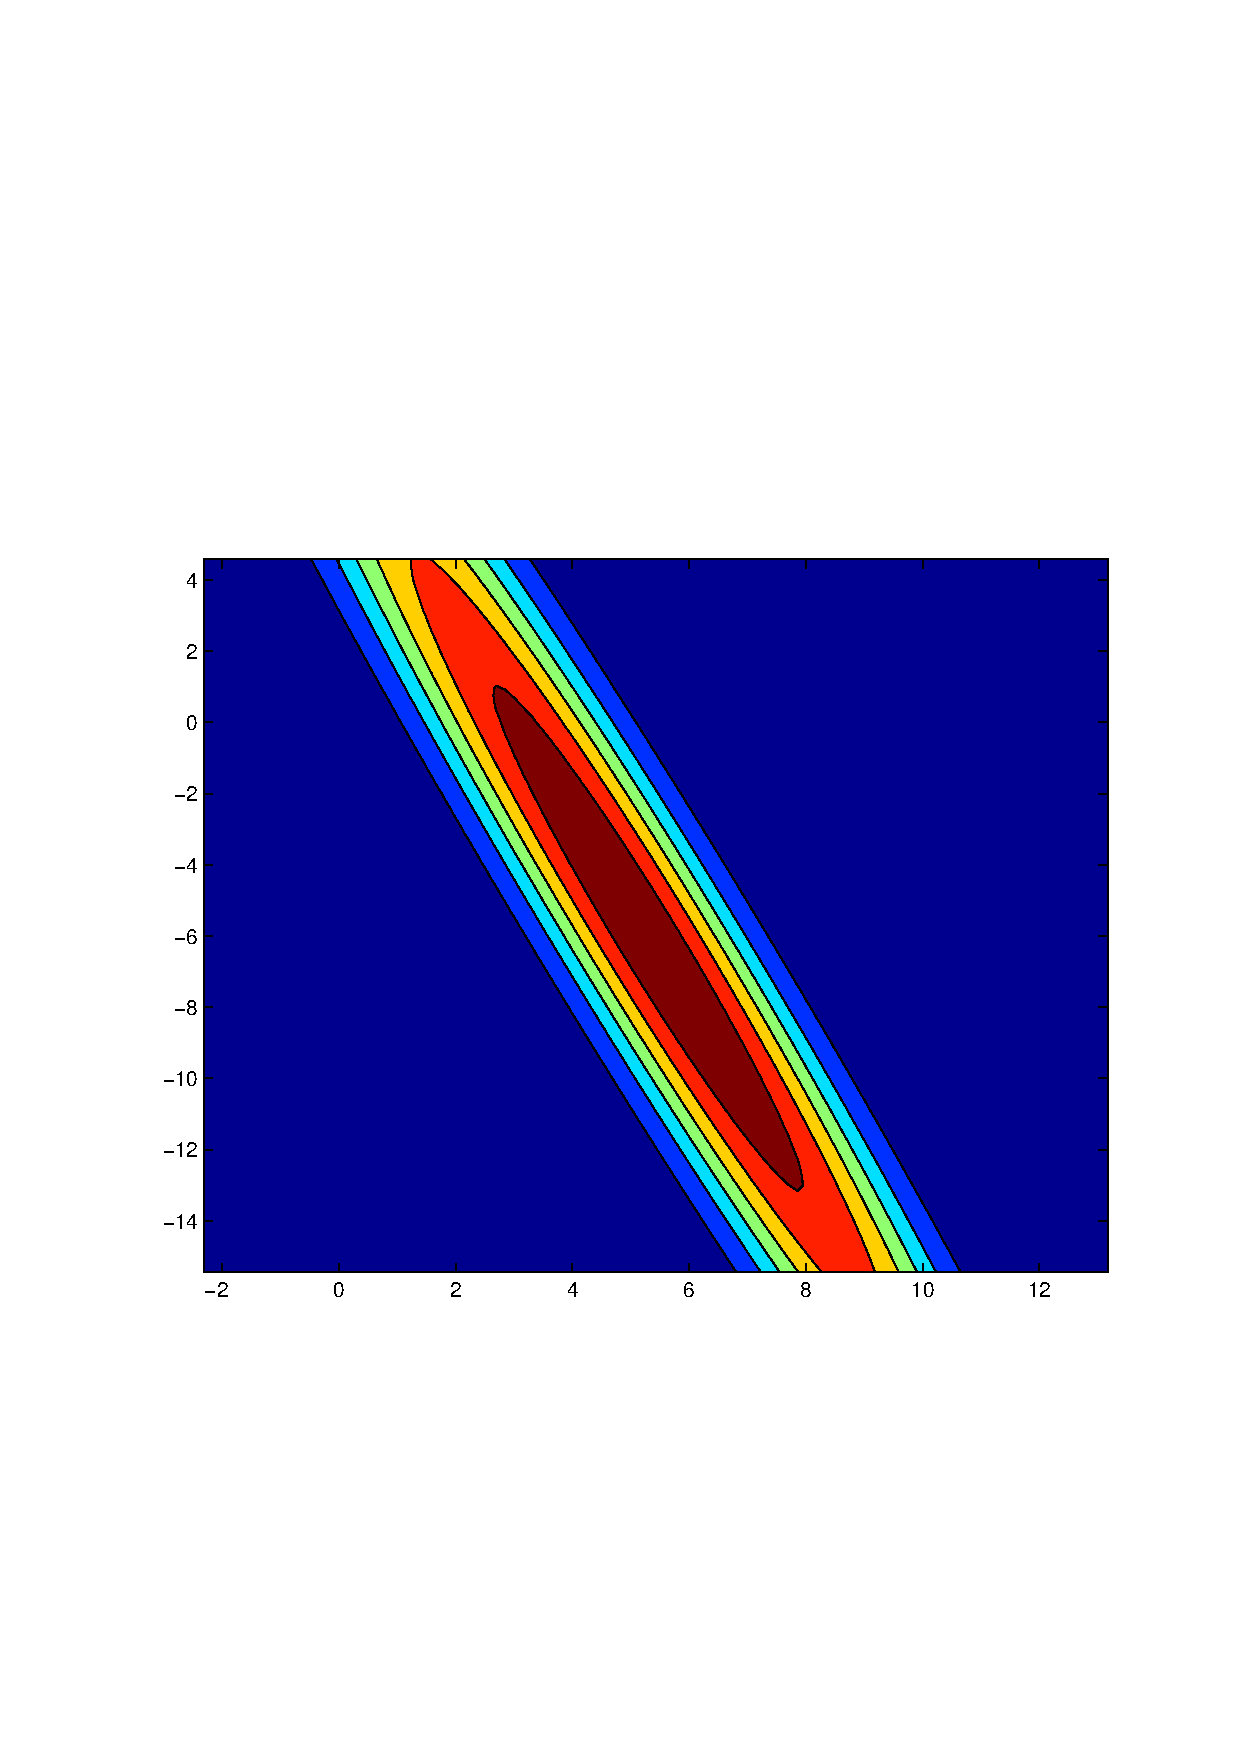
\includegraphics[trim = 150px 100px 150px 70px, clip=true,width=\textwidth]{VC1.jpg}
        \end{subfigure}
       
         \begin{subfigure}[b]{70 px}
                \includegraphics[trim = 150px 100px 150px 70px, clip=true,width=\textwidth]{global2.jpg}
        \end{subfigure}
        ~
         \begin{subfigure}[b]{70 px}
                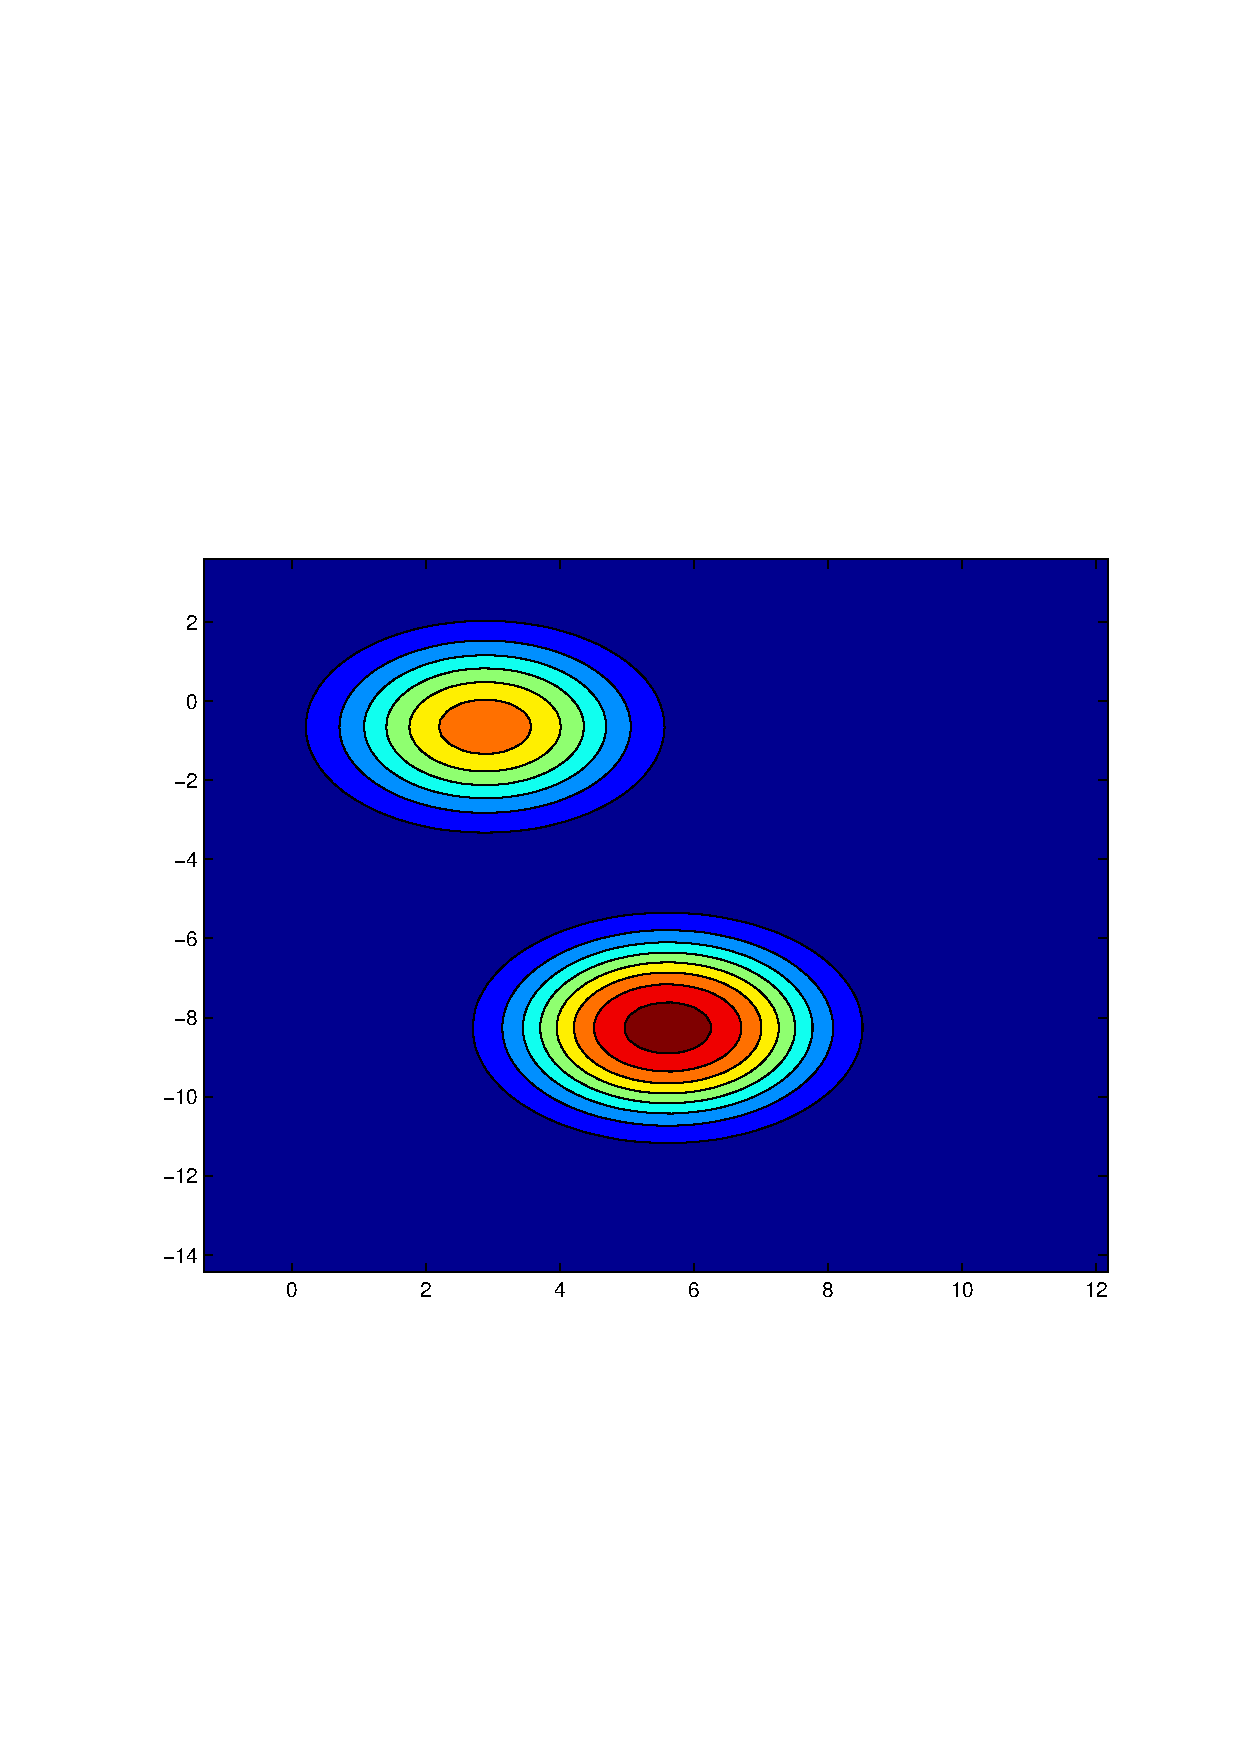
\includegraphics[trim = 150px 100px 150px 70px, clip=true,width=\textwidth]{VL2.jpg}
        \end{subfigure}
        ~
        \begin{subfigure}[b]{70 px}
                \includegraphics[trim = 150px 100px 150px 70px, clip=true,width=\textwidth]{VC2.jpg}
        \end{subfigure}
       
         \begin{subfigure}[b]{70 px}
                \includegraphics[trim = 150px 100px 150px 70px, clip=true,width=\textwidth]{global3.jpg}
        \end{subfigure}
        ~
         \begin{subfigure}[b]{70 px}
                \includegraphics[trim = 150px 100px 150px 70px, clip=true,width=\textwidth]{VL3.jpg}
        \end{subfigure}
        ~
        \begin{subfigure}[b]{70 px}
                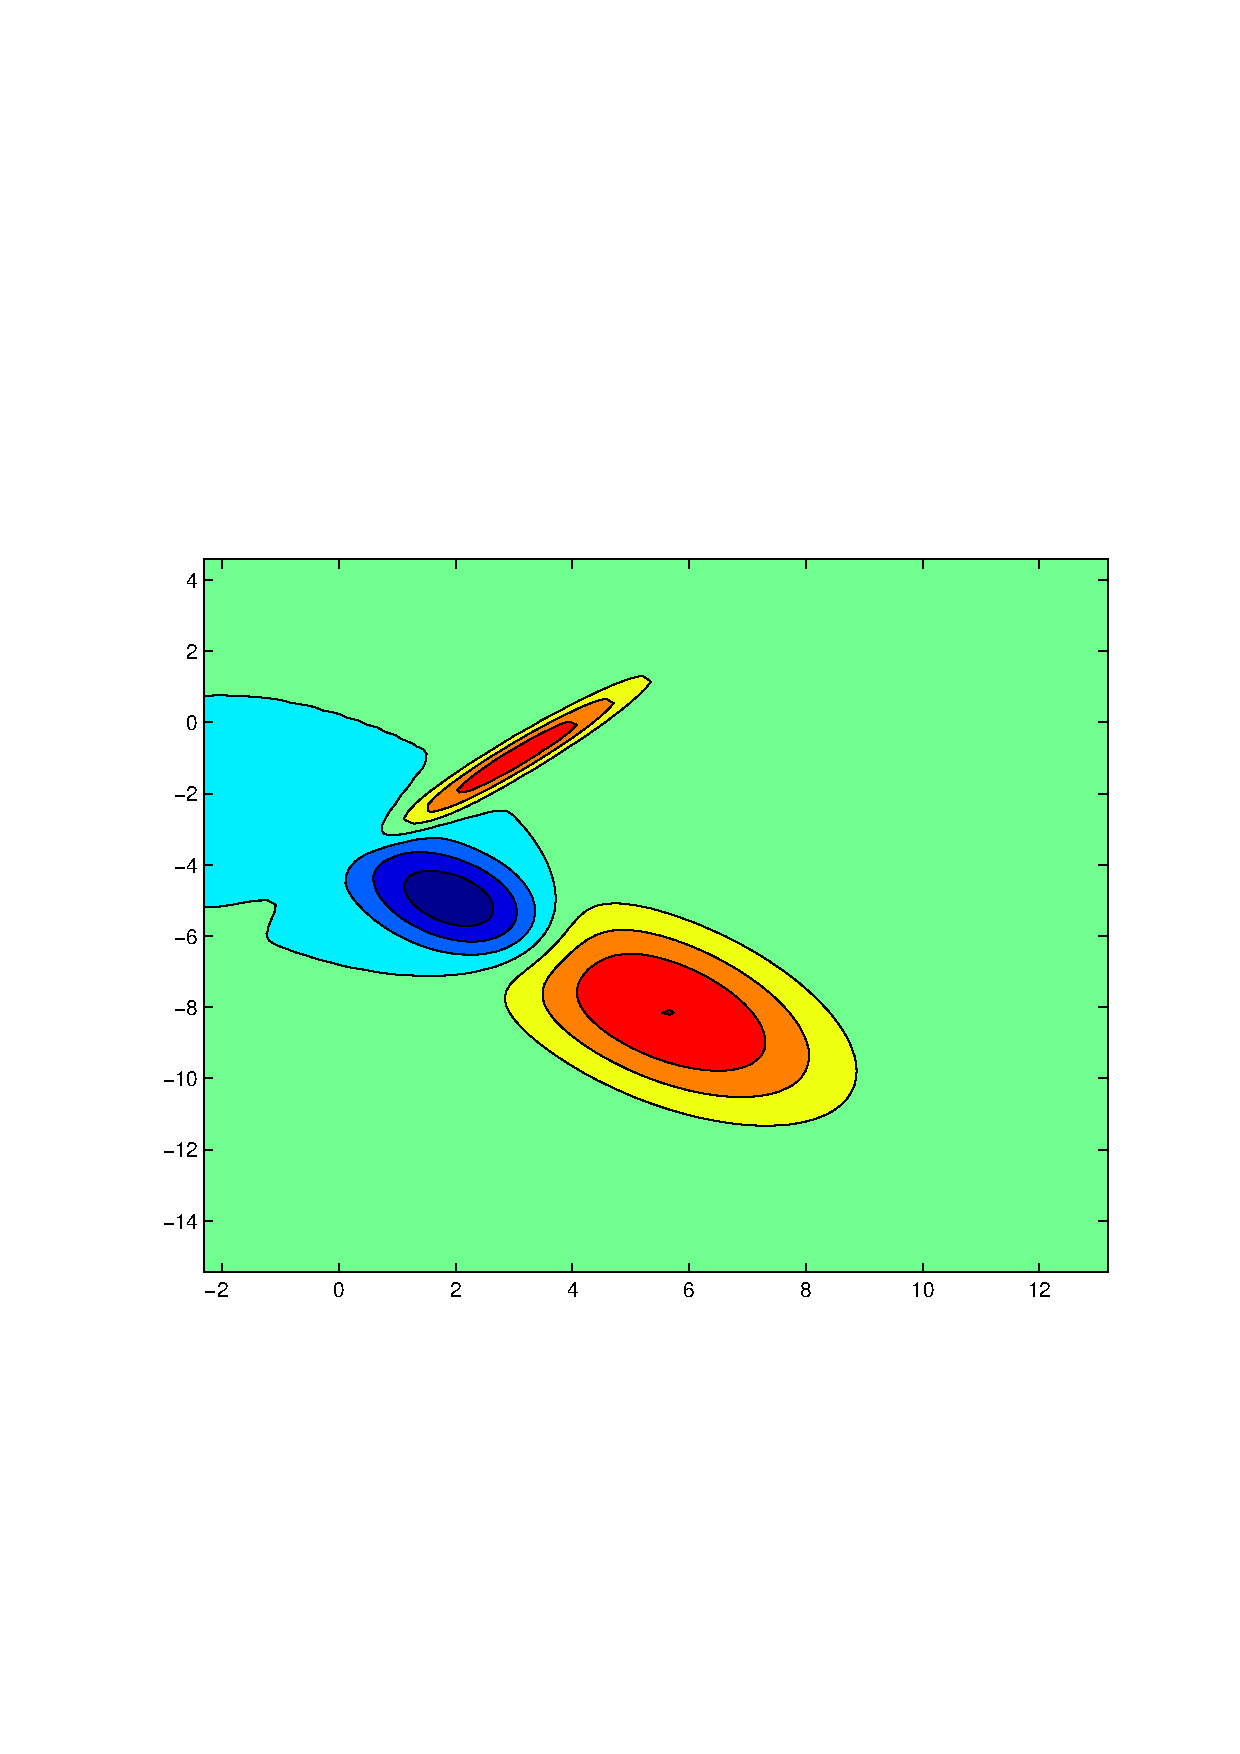
\includegraphics[trim = 150px 100px 150px 70px, clip=true,width=\textwidth]{VC3.jpg}
        \end{subfigure}
       
         \begin{subfigure}[b]{70 px}
                \includegraphics[trim = 150px 100px 150px 70px, clip=true,width=\textwidth]{global4.jpg}
                \caption{Global length scale}
        \end{subfigure}
        ~
         \begin{subfigure}[b]{70 px}
                \includegraphics[trim = 150px 100px 150px 70px, clip=true,width=\textwidth]{VL4.jpg}
                \caption{Variable length scale}
        \end{subfigure}
        ~
        \begin{subfigure}[b]{70 px}
                \includegraphics[trim = 150px 100px 150px 70px, clip=true,width=\textwidth]{VC4.jpg}
                \caption{Variable covariance}
        \end{subfigure}
               
        \caption{A comparisons between different sparse GP approaches with 1 to 4 basis functions (top to bottom) using (a) a global length scale, (b) variable length scales and (c) variable covariances }
        \label{fig-toy-comparison}
\end{figure}

\subsection{Linear Regression Prior}

GPs tend to perform well in interpolation but not as well in extrapolating. The regression function will fall back to the prior mean in areas where there is no training data. A common preprocessing technique is to subtract the mean of the output prior to training then adding it to the prediction of the model. Another way is to subtract a simple linear regression model and train the GP to learn the variation from that. This way, the GP will fall back to the linear regression prediction as a way of last resort instead of falling back to zero. We can incorporate this directly into the optimization objective instead of having it as a separate preprocessing step by redefining $K$ as a concatenation of the linear and non-linear features, or setting $K=[K|X|\underset{n}{1}]$. Furthermore, the regularization matrix in \eqref{eq-linear-regression-objective-rectangular} can be modified so that it penalizes for learning high coefficients for the non-linear terms but no or little cost for learning linear terms by setting the corresponding elements in the diagonal of $I$ to 0, or the last $d+1$ elements. Therefore, as $\sigma_{n}^{2}$ goes to infinity, the model will get closer to a simple linear regression model.

\subsection{Cost Sensitive Learning}

So far the objective is to minimize the sum of squared errors, which is a suitable objective for most applications. However, this objective is naturally biased to the mean of the input and output distribution, therefore sacrificing data samples in less represented regions of the space. This is not always a desired effect, ideally we would like to train with well balanced data to avoid any bias, but this is a luxury that we often do not have. A common technique is to either over-sample or under-sample the data to achieve balance \cite{}. In under-sampling, samples are removed from highly represented regions to achieve balance, over-sampling on the other hand duplicates under represented samples. Both approaches come with a cost, in the former good data is being wasted and in the latter more computation is introduced due to the data size increase. In this paper, we used what is known as cost-sensitive learning, which increases the error cost for low represented samples to mimic over-sampling balance. In classification tasks, a cost per sample is introduced such that the sum of the weights for each class are equal. In regression tasks, the output can be either discritized and treated as classes for the purpose of cost assignment, or a probability function is fitted to the output then samples are weighted in proportion to their inverse probability. After the weights have been assigned, they can be incorporated directly into the objective as follows:

\begin{equation}
\label{eq-weighted-linear-regression-objective}
\begin{array}{lcl}
\underset{w}{\text{min}} &\frac{1}{2}\left ( Kw-y \right )^{T} W\left( Kw-y \right )+\frac{1}{2}\sigma_{n}^{2}w^{T}w
\end{array}
\end{equation}

The only difference between the objectives in \eqref{eq-linear-regression-objective} and \eqref{eq-weighted-linear-regression-objective} is the introduction of the diagonal matrix $W$, where each element $W_{ii}$ is the corresponding cost for sample $i$. The first term in \eqref{eq-weighted-linear-regression-objective} is a matrix form for a weighted sum of squares $\sum_{i=1}^{n}W_{ii}\left(K_{i,*}w-y_{i}\right)^{2}$. The solution to can be found analytically as follows:

\begin{equation}
\label{eq-weighted-linear-regression-objective-rectangular}
w = \left(K^{T}WK+I\sigma_{n}^{2} \right)^{-1}K^{T}Wy
\end{equation}

\section{Application to Photometric Redshift Estimation}
\label{sec-application}

Here we consider the problem of redshift estimation from photometric data. The aim is to predict the spectroscopic redshift from the magnitudes of different colour bands omitted by a source using photometry, the light for each band is filtered to measure the magnitude of a certain wavelength range. We specifically target the photometric configuration designed for the Euclid Space Mission, namely the g, r, i, z, RIZ, Y, J and H bands and their associated expected errors. 

\subsection{Dataset}
\label{sec-dataset}

The dataset consist of the g, r, i, z, RIZ, Y, J and H magnitudes for 156,904 simulated sources along with their spectroscopic redshift. They cover a redshift range of $0.2 \le z_{spec} \le 2$ to target the requirement set by the Euclid Space Mission. All sources with any missing measurement in any of their detectors were removed prior to training. Not limits on any of the bands were used, although some will be explicitly removed to test the extrapolation performance of the models. The distribution of the bands and the spectroscopic redshift are provided in Figures \ref{fig-bands-hostograms} and \ref{fig-zpec-hostogram} respectively. For all experiments reported in this paper, we ignore the error bars associated with each band and train only on the magnitudes. In all experiments reported in this paper, the data is preprocessed using Principle Component Analysis (PCA) \cite{} to de-correlate the features prior to learning. De-correlation is known to accelerate the convergence rate specially when using a logistic-type kernel machines like Neural Networks \cite{}, and a similar effect is noticed with the squared exponential kernel here.

\begin{figure*}
       \centering
       \includegraphics[width=0.75\textwidth]{bands.jpg}
        \caption{The magnitude distribution for each band in the dataset.} 
       \label{fig-bands-hostograms}
\end{figure*}

\begin{figure}
       \centering
       \includegraphics[width=\columnwidth]{zpec.jpg}
        \caption{The spectroscopic redshift distribution in the dataset.} 
       \label{fig-zpec-hostogram}
\end{figure}

\section{Experiments and Results}
\label{sec-experiments}

Five algorithms are considered to model the data, Artificial Neural Networks (ANN), GP with low rank approximation or stableGP, sparse GP with global length scale (GP-GL), GP with variable length scale (GP-VL) and  GP with variable covariances (GP-VC). For ANN, a single layer network is used with hyperbolic tangent hidden activations and linear output activations, for low rank approximation we use the SR-VP method proposed in \cite{}. In subsequent tests, the variable $m$ refers to the number of hidden units in ANN, the rank in stableGP, and the number of basis functions in GP-GL, GP-VL and GP-VC. The data was split into \%90 for training and \%10 for testing, the following performance measures on the test set are reported for each experiment:

\begin{itemize}
  \item $\Delta z_{\phantom{norm}} = \sqrt{\frac{1}{n}\sum_{i=1}^{n}\left(z_{spec}-z_{phot}\right)^{2}}$
  \item $\Delta z_{norm} = \sqrt{\frac{1}{n}\sum_{i=1}^{n}\left(\frac{z_{spec}-z_{phot}}{1+z_{spec}}\right)^{2}}$
\end{itemize}

$\Delta z$ is the standard Root Mean Squared Error (RMSE), while $\Delta z_{norm}$ is a normalized version that weighs low redshift objects more aggressively than higher redshift objects. The scientific goal of the Euclid mission is to reach a $\Delta z_{norm} \le 0.05$

\subsection{Modelling Performance}

In the first test, all models were trained using a fixed $m=10$ to cross compare the performance of the methods using the same number of basis functions. The number of basis was set deliberately low to highlight the modelling capabilities of each algorithm, as for large values of $m$ the performance gap between the algorithms is very small to distinguish the difference. The standard sum of squared objective was used , without cost sensitive training or assuming a linear regression model as a prior. The $z_{spec}$ vs $z_{phot}$ density scatter plots are shown in Figure \ref{fig-experiment-1} and their performance scores are reported in Table \ref{table-experiment-1}

\begin{figure}
        \centering
        \begin{subfigure}[b]{110px}
                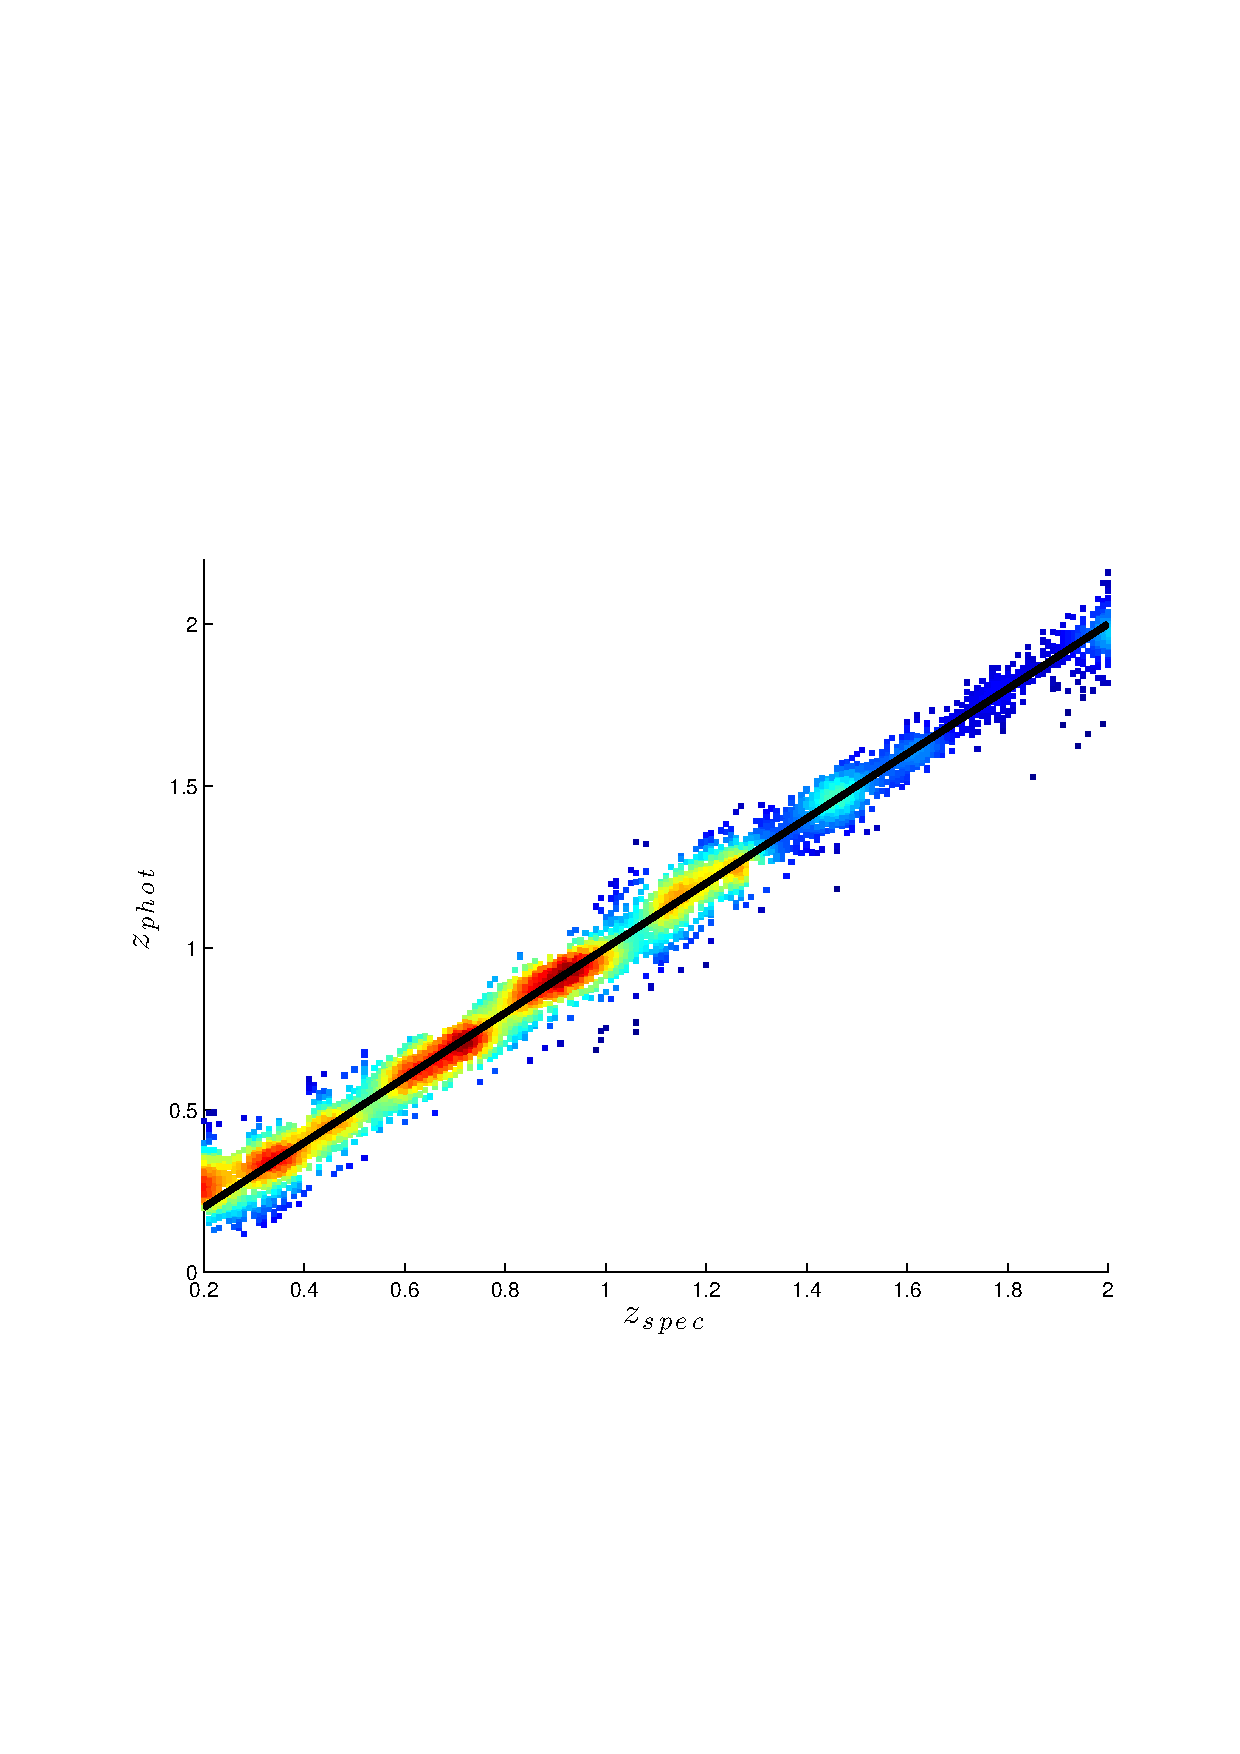
\includegraphics[trim = 35px 15px 50px 25px, clip=true,width=\textwidth]{ANN.jpg}
                \caption{ANN}
        \end{subfigure}
        ~
        \begin{subfigure}[b]{110px}
                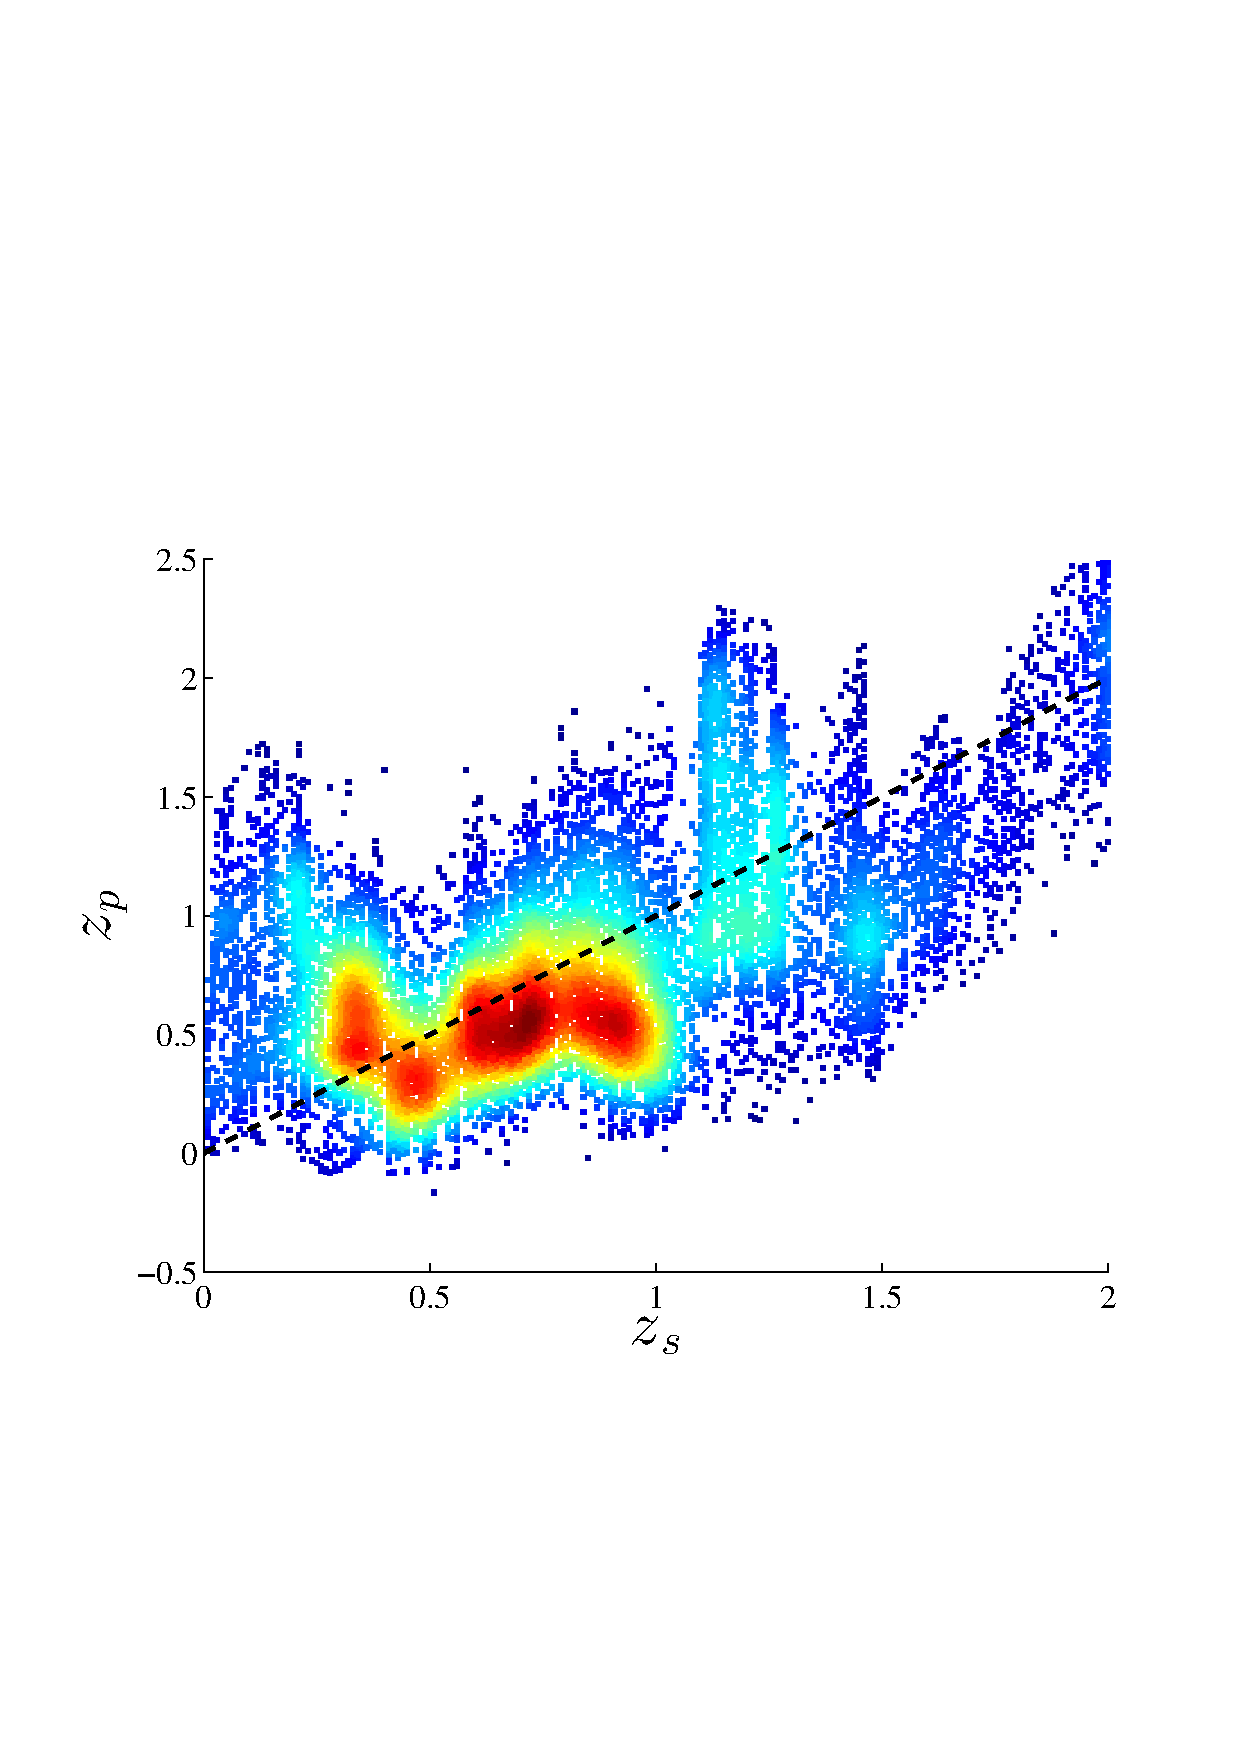
\includegraphics[trim = 35px 15px 50px 25px, clip=true,width=\textwidth]{stableGP.jpg}
                \caption{stableGP}
        \end{subfigure}
        ~
        \begin{subfigure}[b]{110px}
                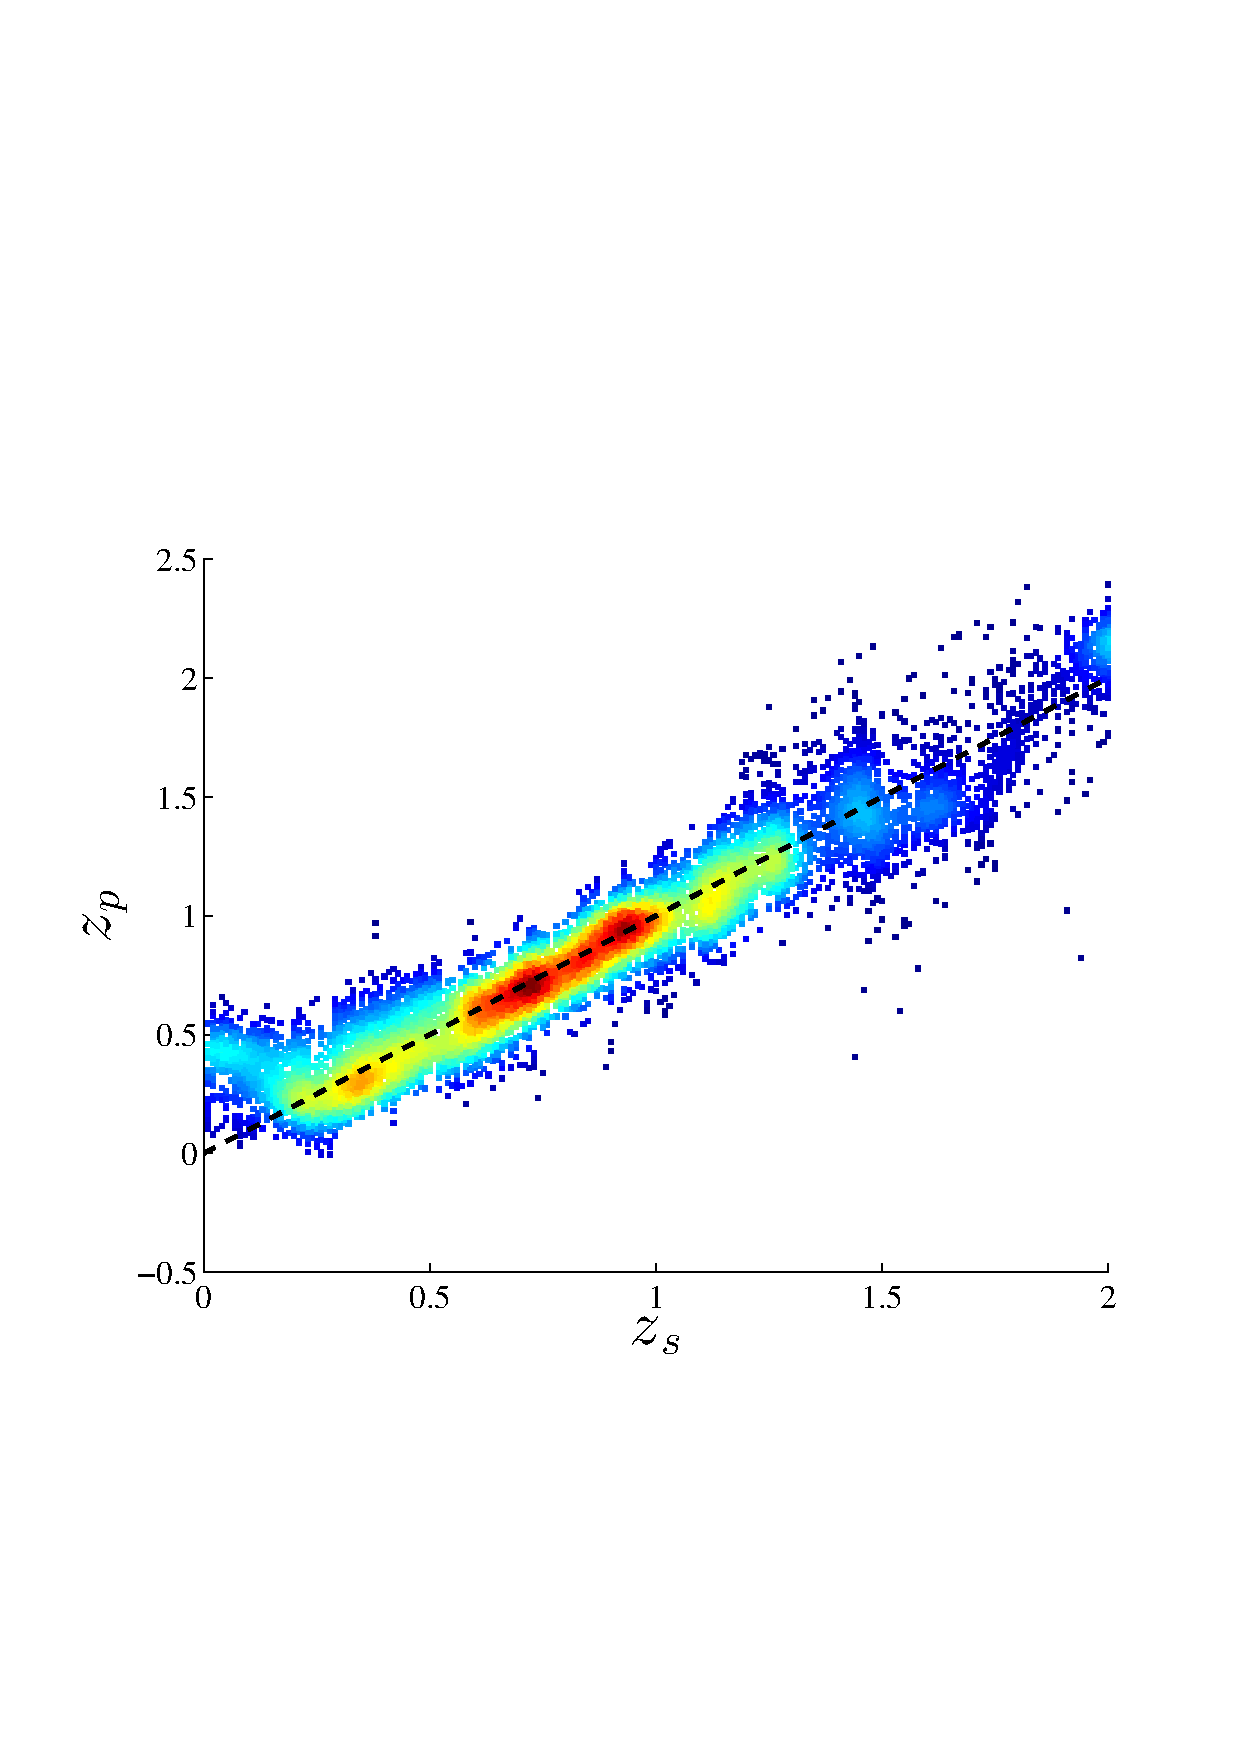
\includegraphics[trim = 35px 15px 50px 25px, clip=true,width=\textwidth]{GPGL.jpg}
                \caption{GP-GL}
        \end{subfigure}
        ~
        \begin{subfigure}[b]{110px}
                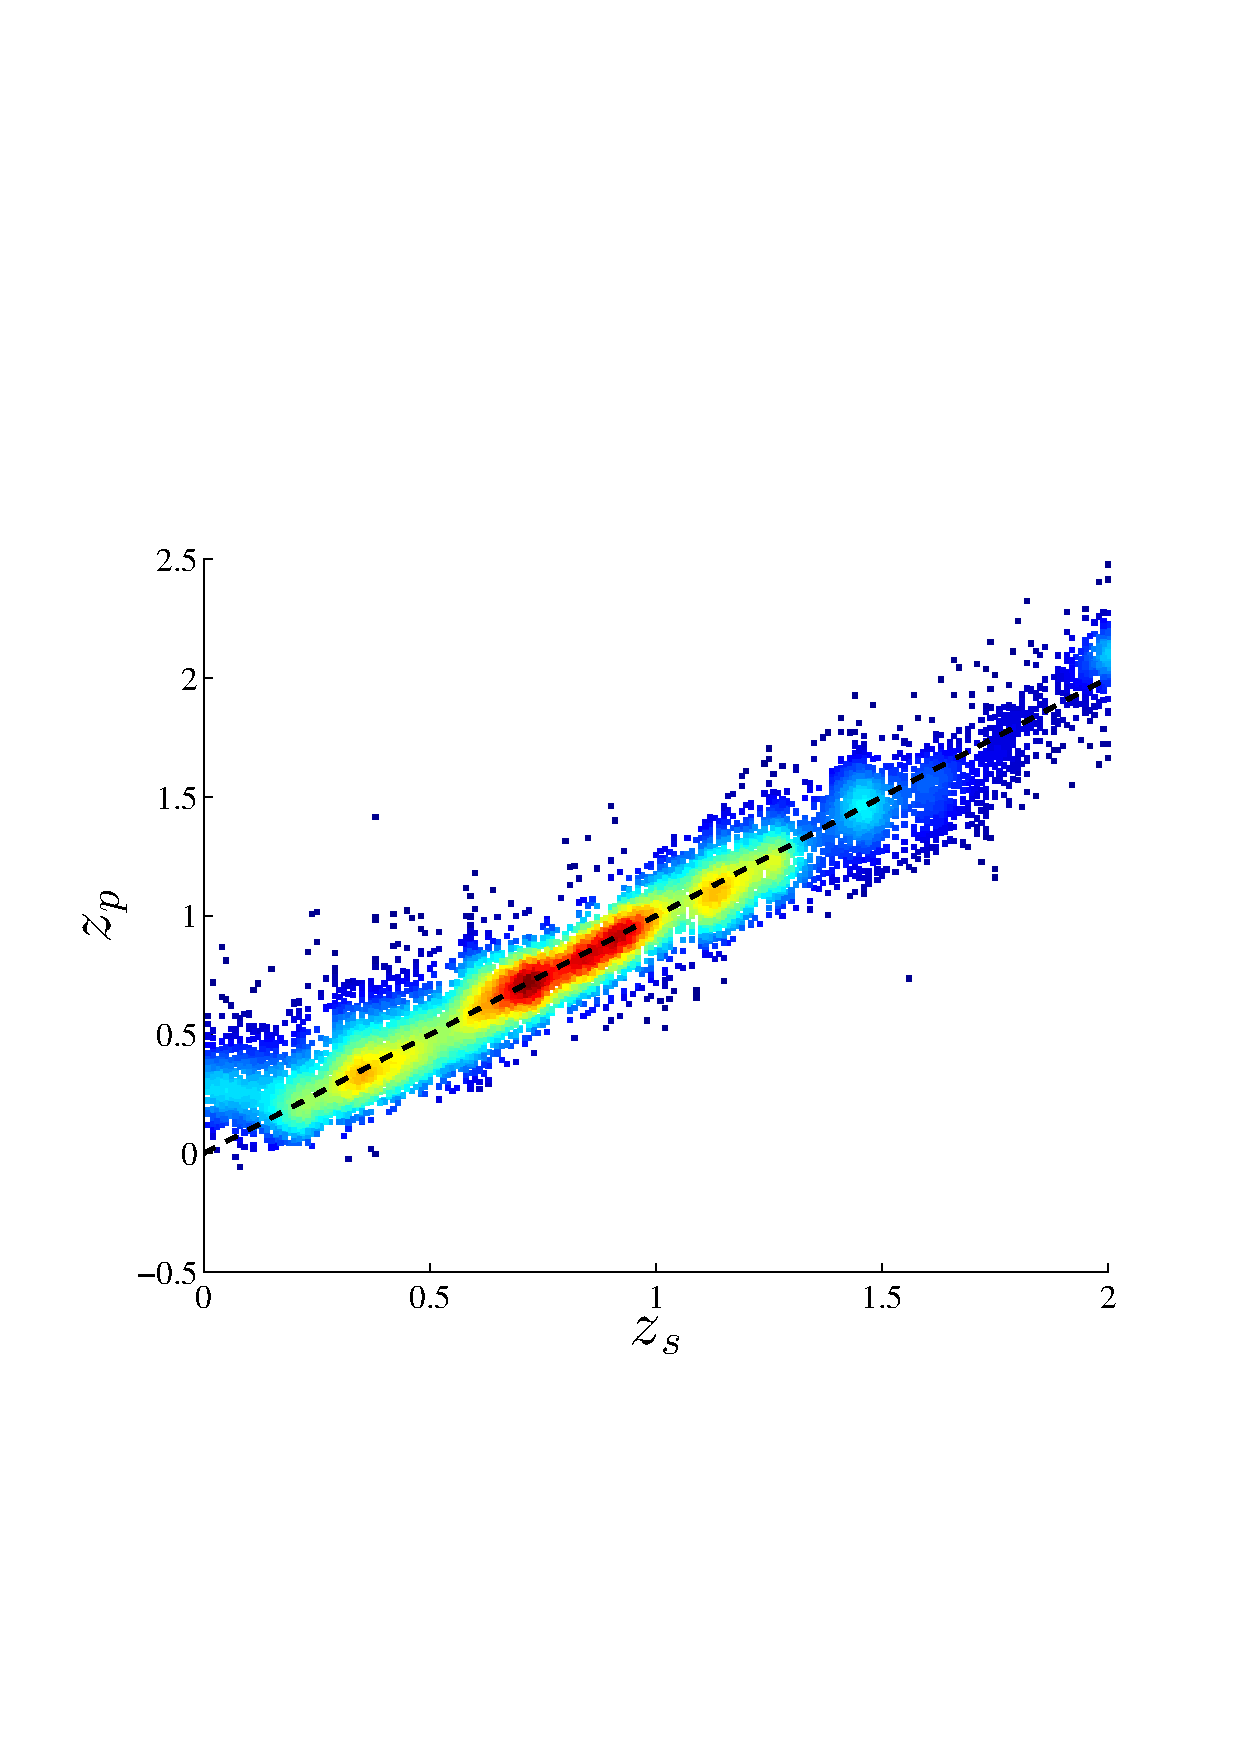
\includegraphics[trim = 35px 15px 50px 25px, clip=true,width=\textwidth]{GPVL.jpg}
                \caption{GP-VL}
        \end{subfigure}
        ~
        \begin{subfigure}[b]{110px}
                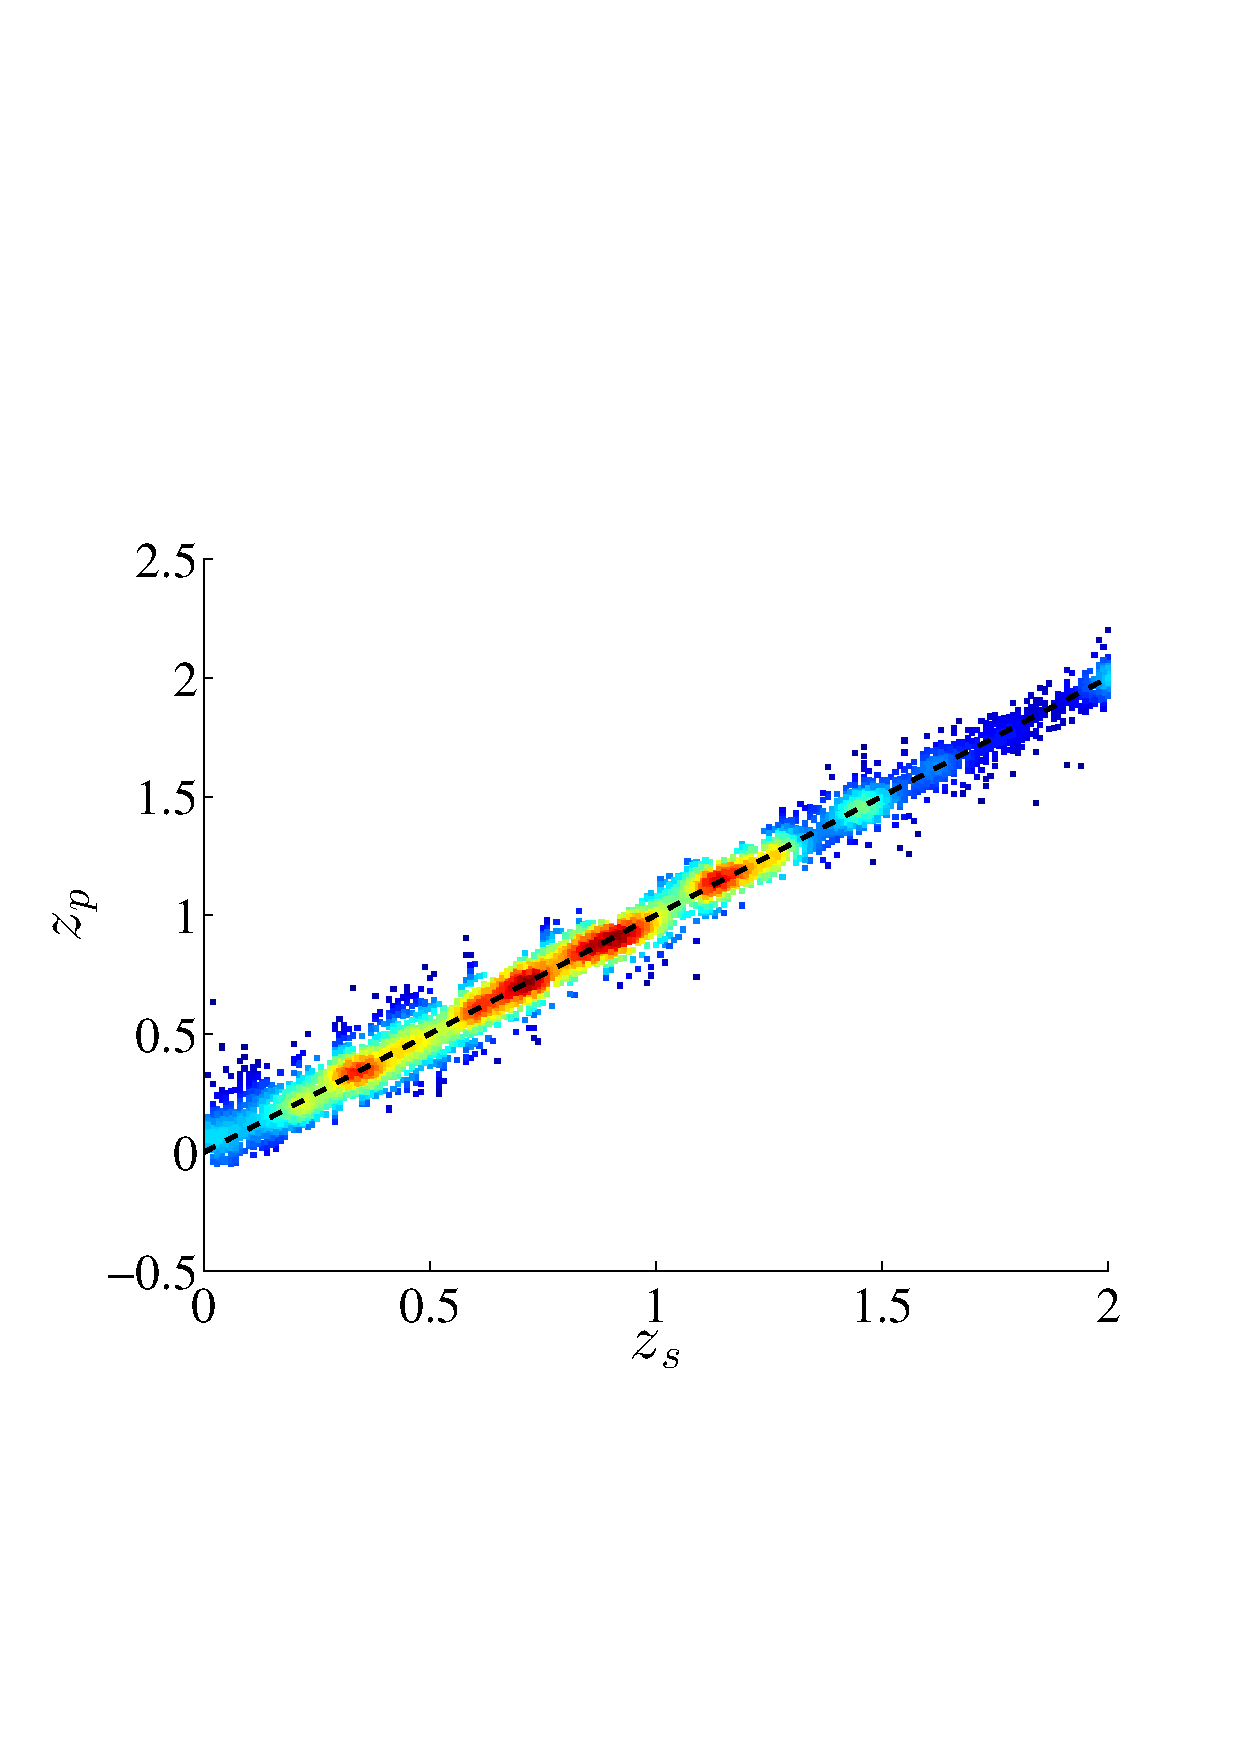
\includegraphics[trim = 35px 15px 50px 25px, clip=true,width=\textwidth]{GPVC.jpg}
                \caption{GP-VC}
        \end{subfigure}
        
        \caption{Scatter density plots of the true $z_{spec}$ vs the predicted $z_{phot}$ for (a) ANN, (b) stableGP, (c) GP-GL, (d) GP-VL and (e) GP-VC using $m=10$ basis functions}
        \label{fig-experiment-1}
\end{figure}

 \begin{table}
\caption{Performance measures for each algorithm trained using $m=10$ basis functions}
\begin{center}
  \begin{tabular}{| l | c | c | }
     				&	$\Delta z$	&	$\Delta z_{norm}$	\\	\hline
	ANN		&	0.0415		&	0.0251				\\	 
	stableGP	&	0.2138		&	0.1304				\\ 
	GP-GL		&	0.0679		&	0.0415				\\
	GP-GL		&	0.0595		&	0.0370				\\
	GP-VC	&	0.0233		&	0.0134				\\	\hline
  \end{tabular}
  \label{table-experiment-1}
\end{center}
\end{table}

\subsection{Prior Mean}

In this test, the extrapolation performance of the GP-VC model was tested using different prior means, namely a zeros mean, a linear regression mean and learning the linear and non-linear features simultaneously while regularizing the non-linear features more aggressively than linear features. To test this more effectively,  the models were trained using sources with $RIZ<23$ (36,244 objects) and tested on the unseen samples with $RIZ\ge23$, a similar test was also conducted using a split of $RIZ<22$ (15,067 objects). The results are reported in Table \ref{table-RIZ-splits} and the density scatter plots are shown for comparison in Figure \ref{fig-RIZ-splits}. The results from Table \ref{table-RIZ-splits} shows that the ``Joint'' method consistently outperforms the other methods especially when trained with a small sample size as in the $RIZ<22$ case. The Linear regression prior was not always better than the zero prior mean in terms of performance measures, in the $RIZ<22$ case for example, but upon examining the density scatter plots in Figure \ref{fig-RIZ-splits}, the zero mean prior has more systematic and catastrophic errors.

 \begin{table}
\caption{Performance measures for each algorithm trained using $m=10$ basis functions}
\begin{center}
  \begin{tabular}{| l | c | c | c | c | }
  							& 	\multicolumn{2}{|c|}{$RIZ<23$}	& 	\multicolumn{2}{c}{$RIZ<22$} \\ \cline{2-5}
     	Prior					&	$\Delta z$	&	$\Delta z_{norm}$&	$\Delta z$	&	$\Delta z_{norm}$	\\	\hline
	Zero					&	0.0807		&	0.0315				&	0.1436		&	0.0547					\\	 
	Linear Regression	&	0.0393		&	0.0188				&	0.1784		&	0.0689					\\ 
	Joint					&	0.0371		&	0.0167				&	0.0560		&	0.0264					\\	\hline
  \end{tabular}
  \label{table-RIZ-splits}
\end{center}
\end{table}

\begin{figure}
        \centering
        \begin{subfigure}[b]{73px}
                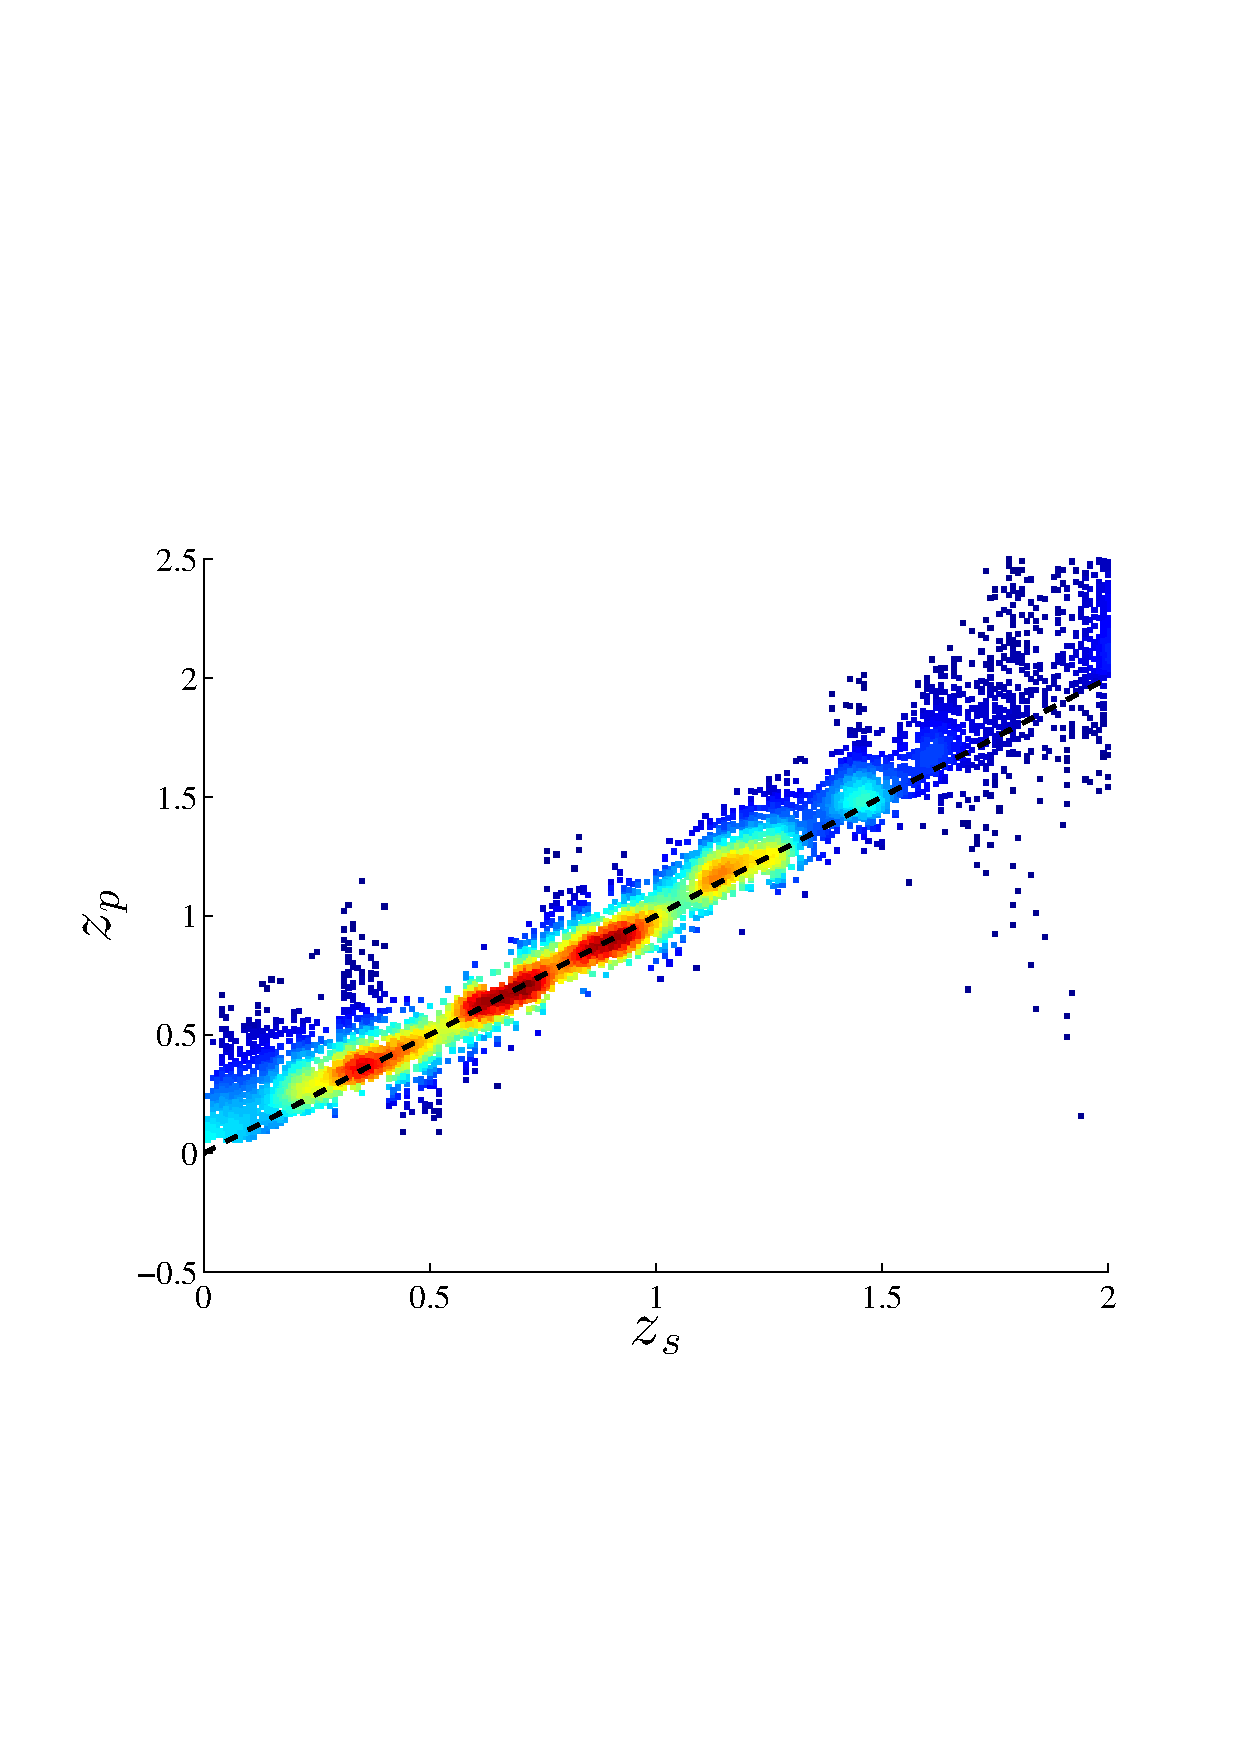
\includegraphics[trim = 35px 15px 50px 25px, clip=true,width=\textwidth]{23_0.jpg}
        \end{subfigure}
        ~
        \begin{subfigure}[b]{73px}
                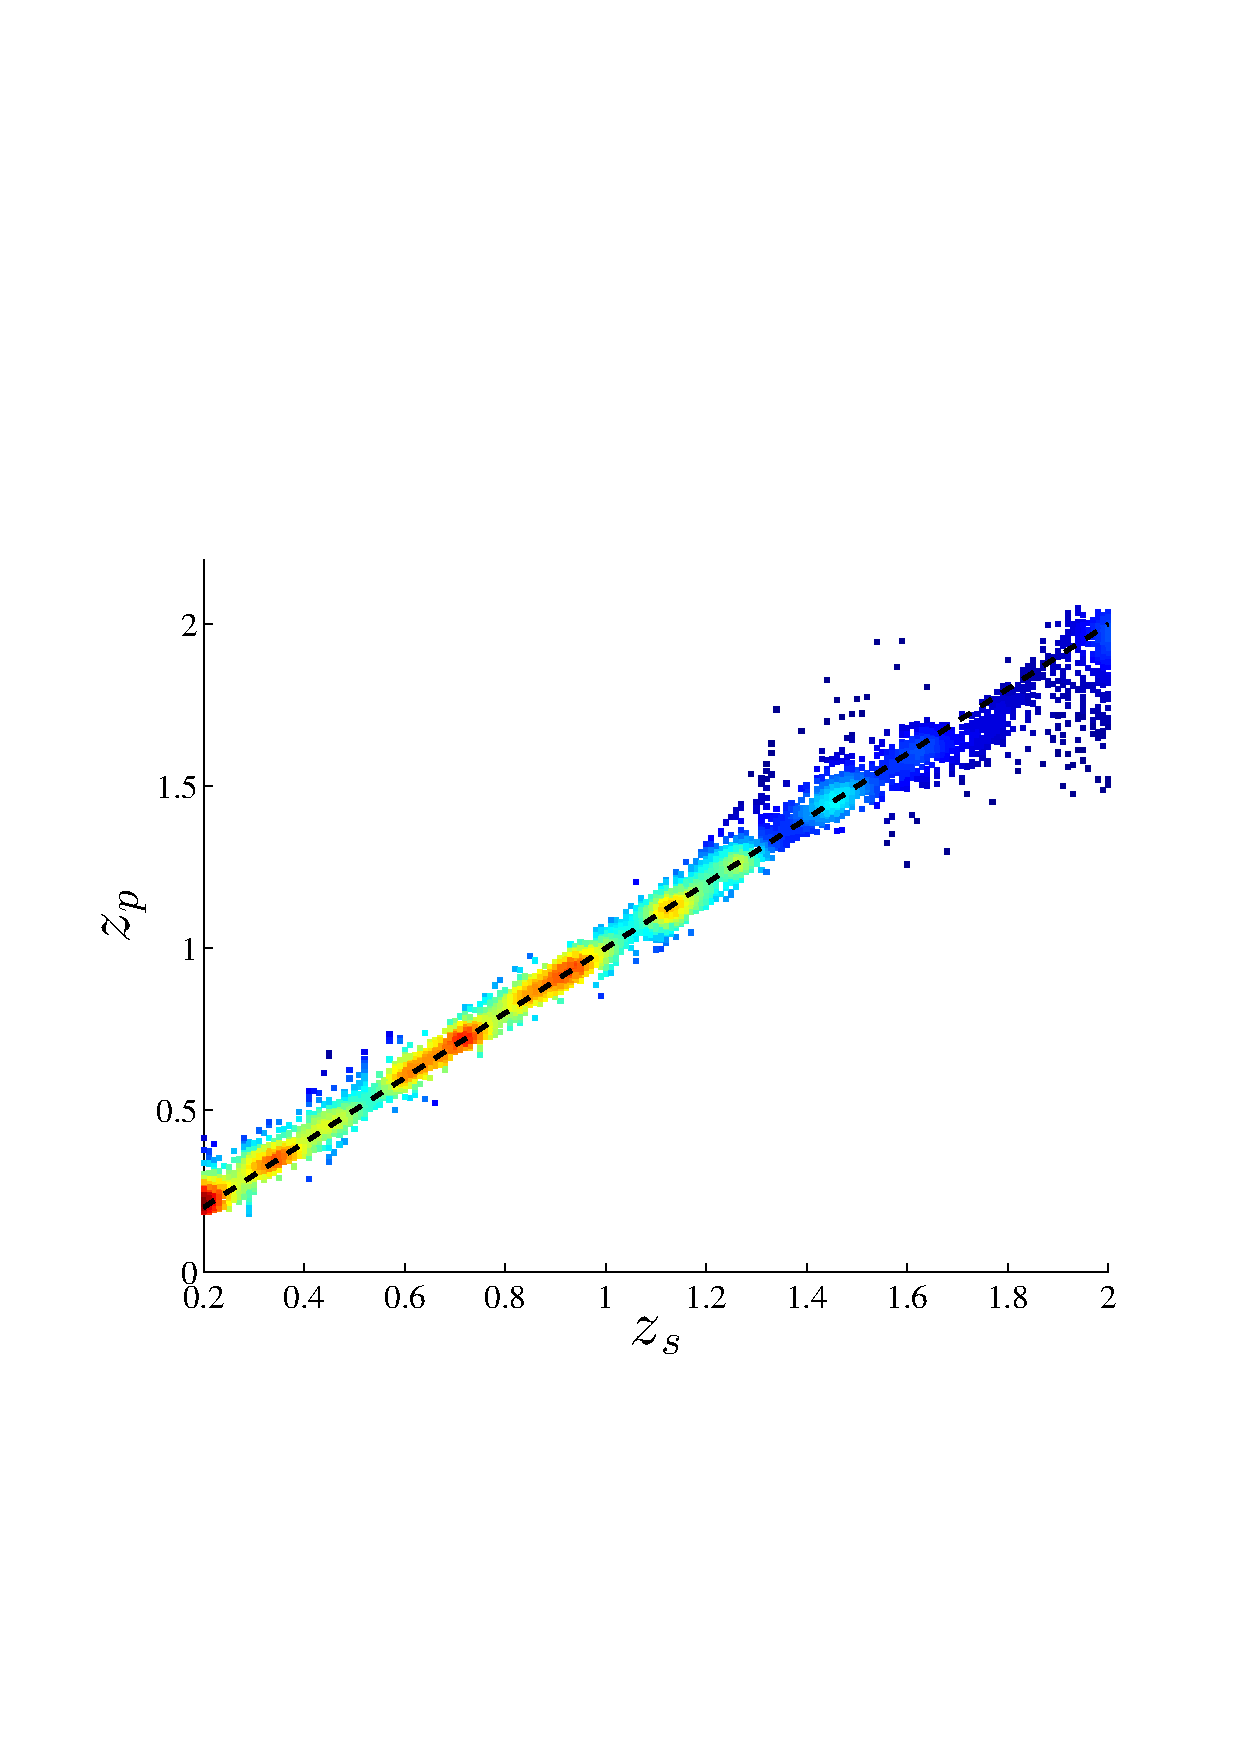
\includegraphics[trim = 35px 15px 50px 25px, clip=true,width=\textwidth]{23_L.jpg}
        \end{subfigure}
        ~
        \begin{subfigure}[b]{73px}
                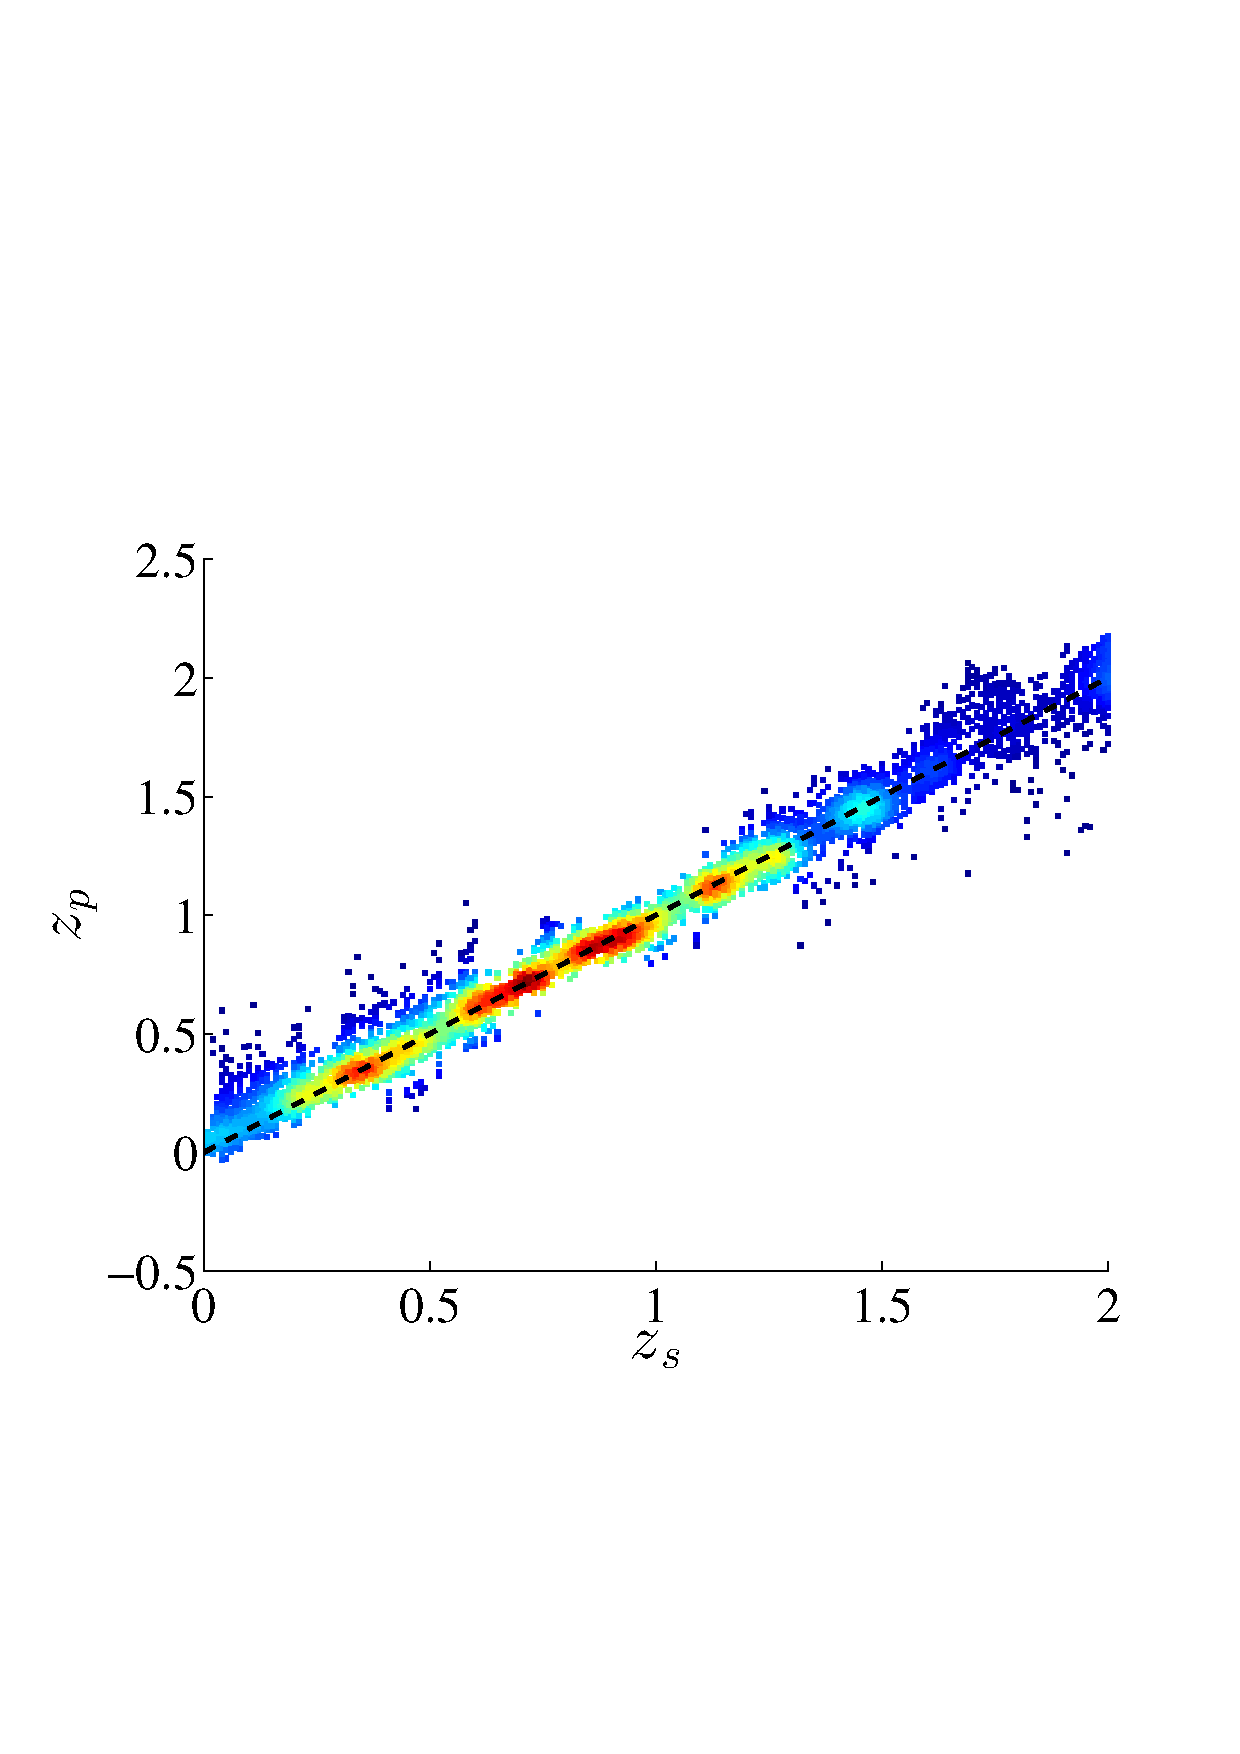
\includegraphics[trim = 35px 15px 50px 25px, clip=true,width=\textwidth]{23_J.jpg}
        \end{subfigure}
        
       \begin{subfigure}[b]{73px}
                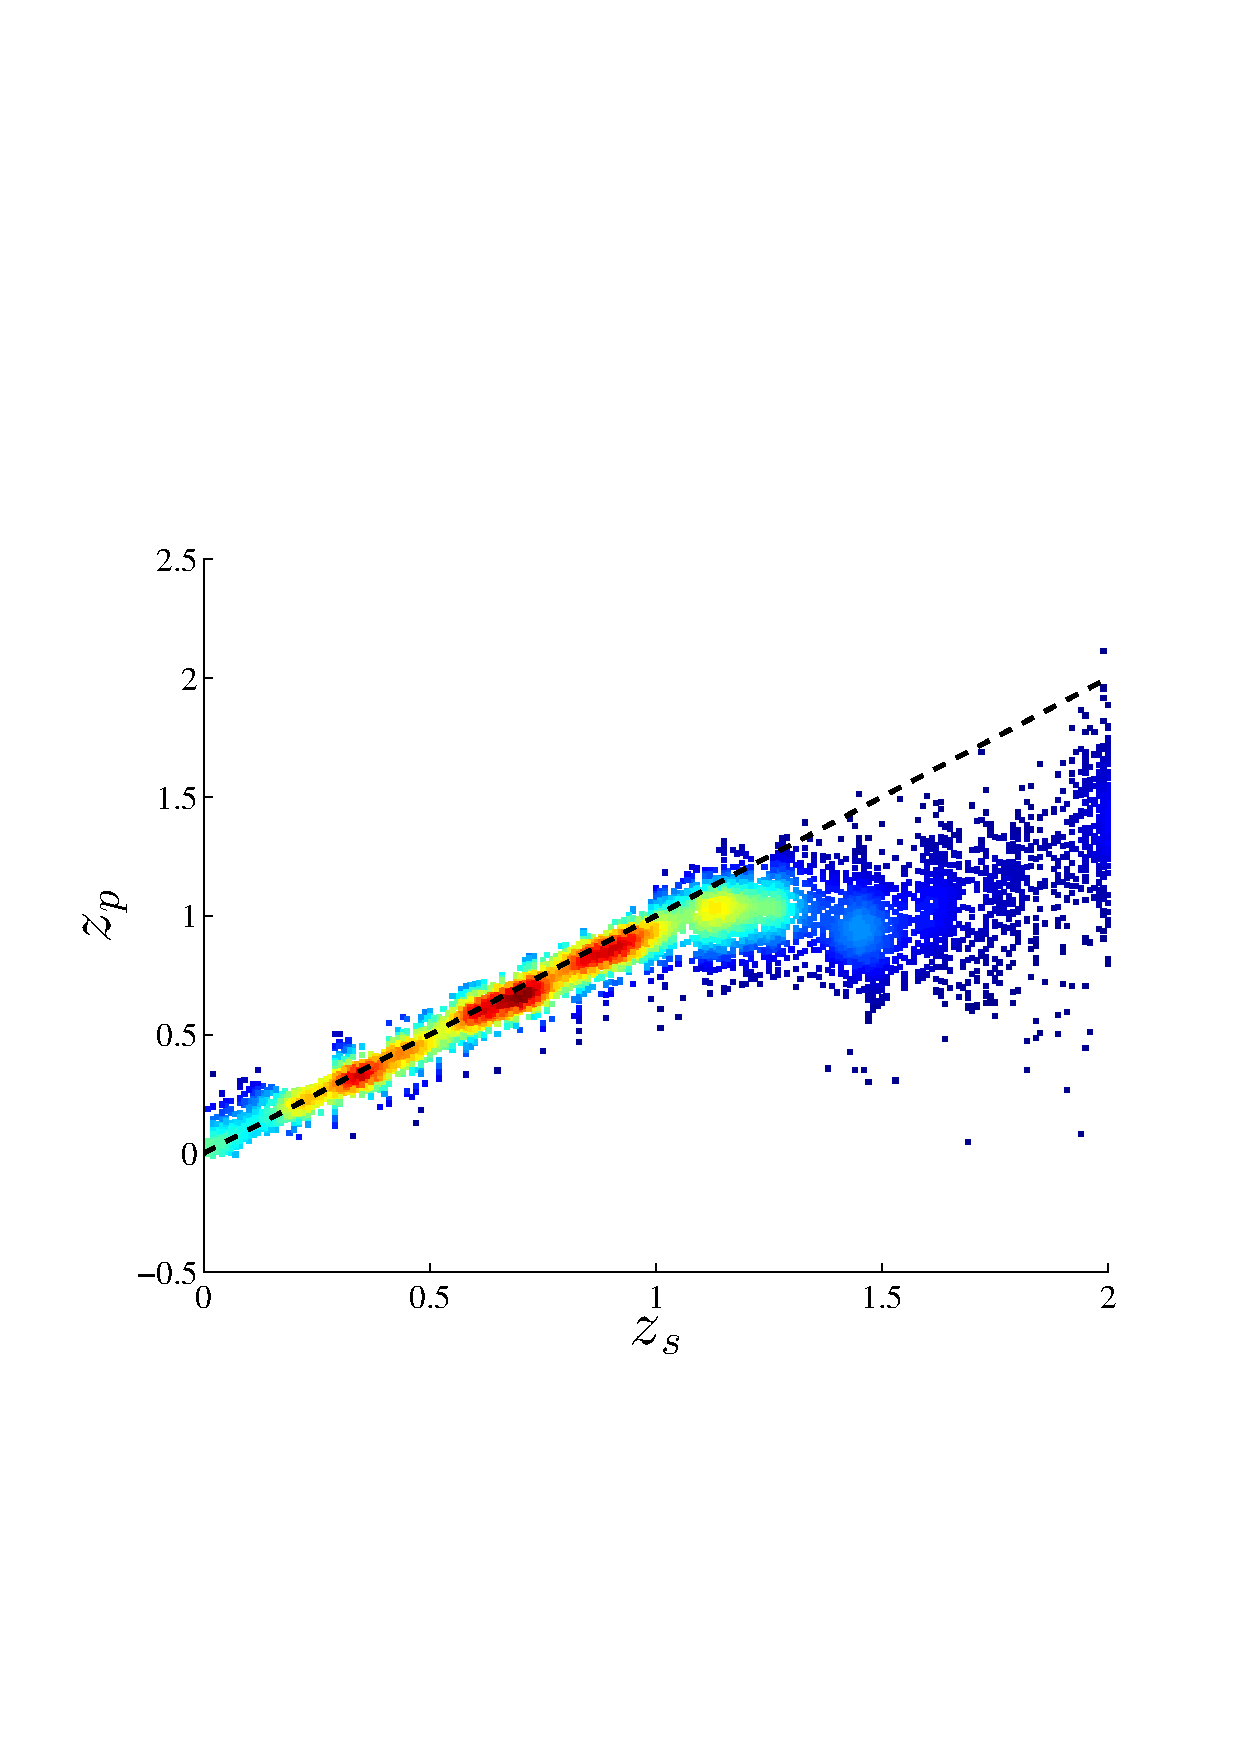
\includegraphics[trim = 35px 15px 50px 25px, clip=true,width=\textwidth]{22_0.jpg}
                \caption{Zero mean}
        \end{subfigure}
        ~
        \begin{subfigure}[b]{73px}
                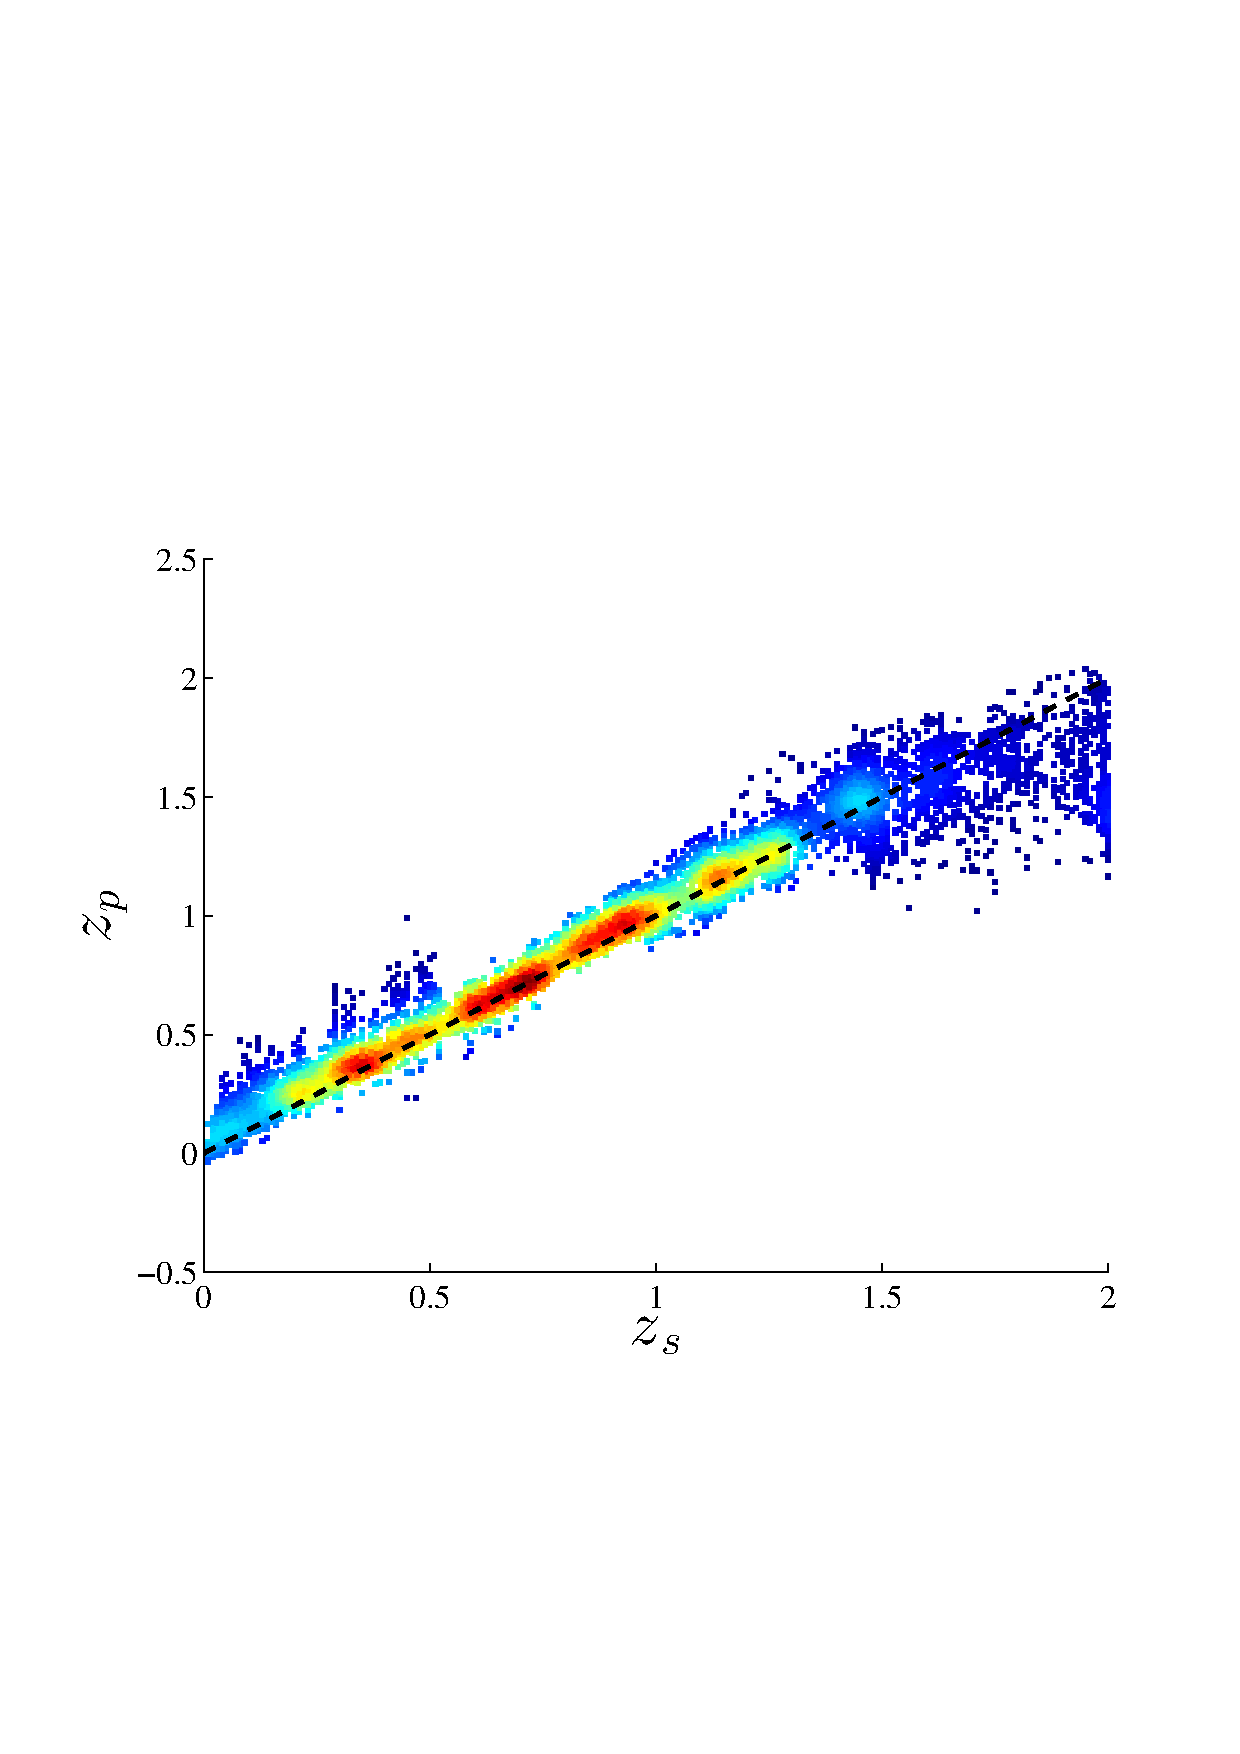
\includegraphics[trim = 35px 15px 50px 25px, clip=true,width=\textwidth]{22_L.jpg}
                \caption{Linear}
        \end{subfigure}
        ~
        \begin{subfigure}[b]{73px}
                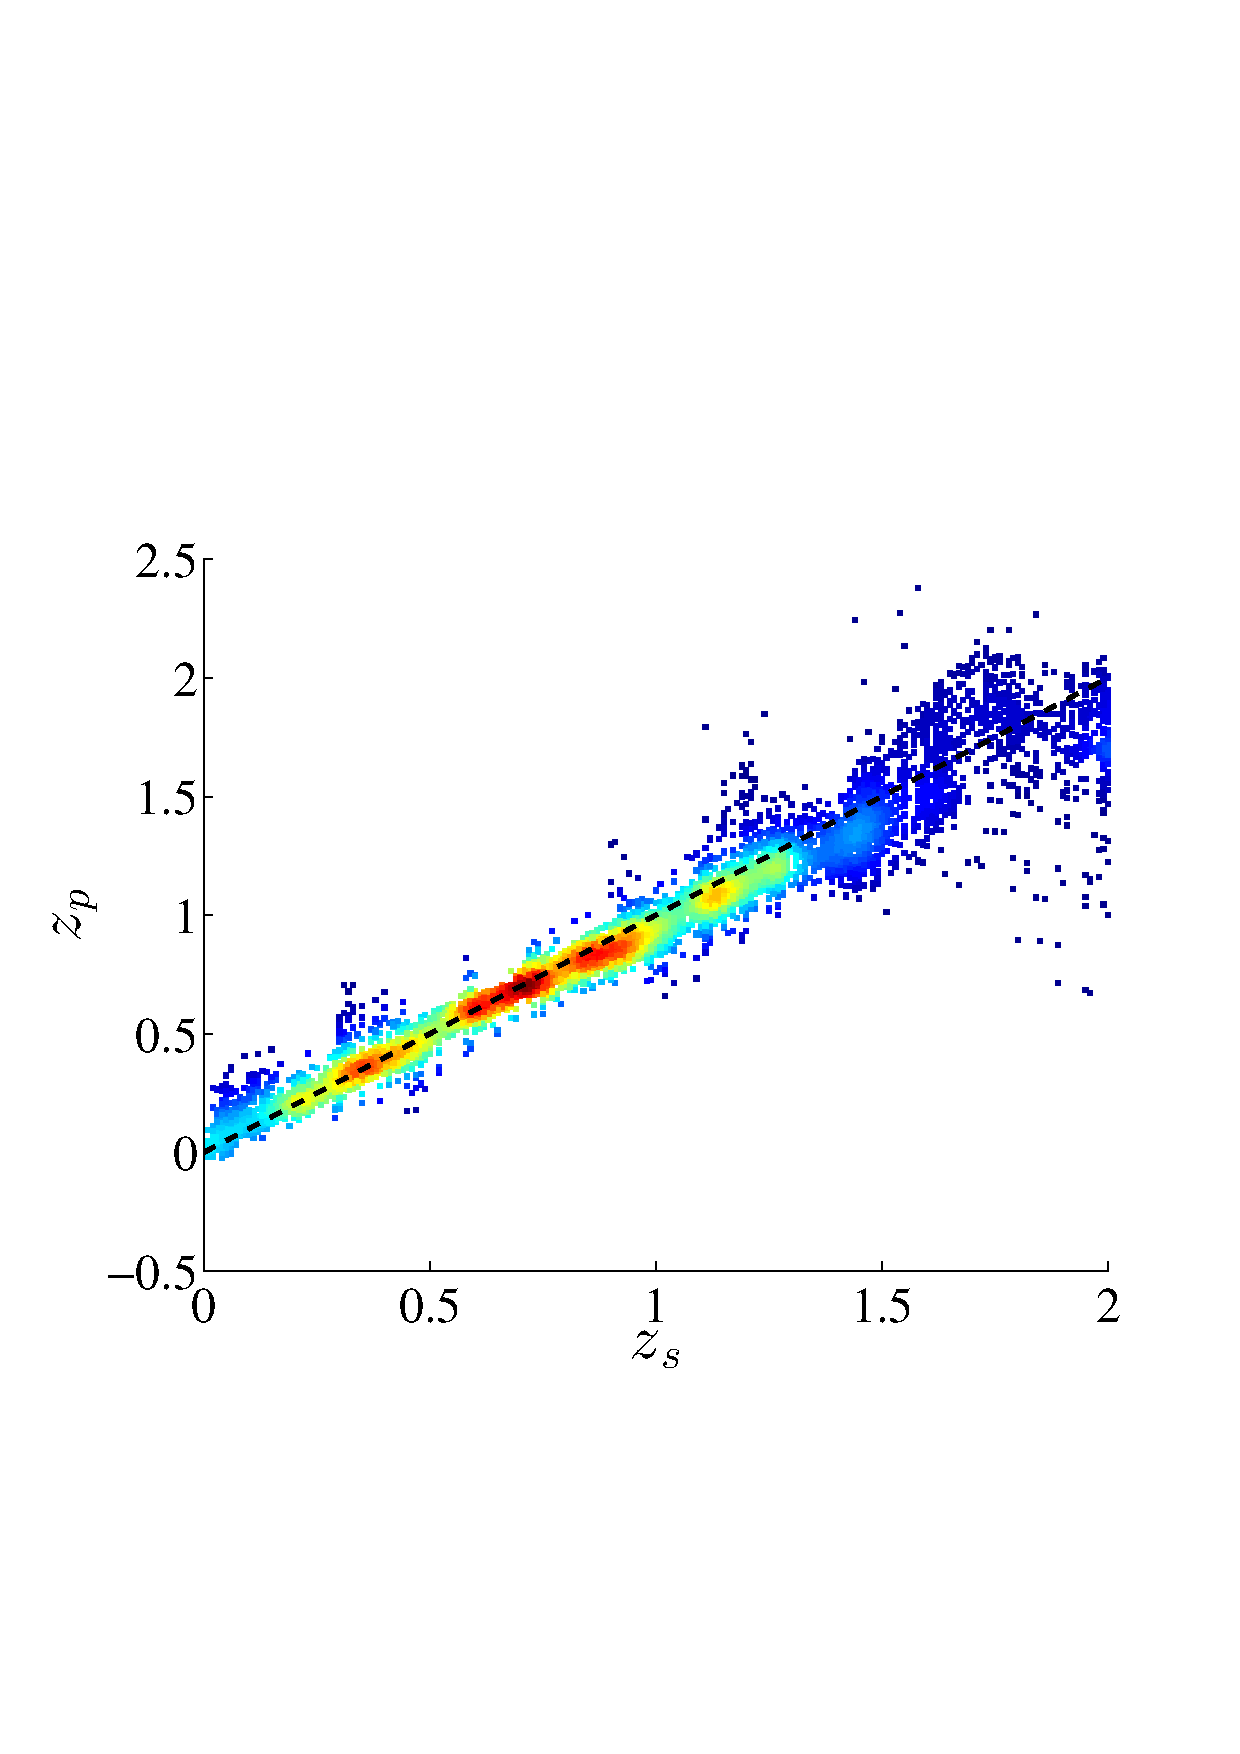
\includegraphics[trim = 35px 15px 50px 25px, clip=true,width=\textwidth]{22_J.jpg}
                \caption{Joint}
        \end{subfigure}
        
        \caption{Density scatter plots of the true $z_{spec}$ vs the predicted $z_{phot}$ after training the GP-VC model with samples with $RIZ<23$ (top) and $RIZ<22$ (bottom) using $m=10$ basis functions with (a) zero mean, (b) linear regression and (c) joint linear and non-linear optimization}
        \label{fig-RIZ-splits}
\end{figure}


\section{Conclusion}
\label{sec-conclusion}

\footnotesize{
\bibliographystyle{mn2e}
\bibliography{biblio.bib}	
}

\end{document}
